% !TEX encoding = UTF-8 Unicode
\documentclass[11pt, a4paper]{article}

\usepackage{todonotes}
\usepackage{subcaption}

% Setup of packages used
\usepackage[onehalfspacing]{setspace}		% One half spacing
\newlength{\stockheight}					% To prevent hyperref warning
\setlength{\stockheight}{\paperheight}		% define \stockheigh
\usepackage{hyperref}					% Hyperlinks on pdf (Should be called before Geometry)
\usepackage[a4paper, 					% Page Layout
                     %showframe,				% This shows the frame
                     includehead,
                     footskip=7mm, headsep=6mm, headheight=4.8mm,
                     marginparsep=2mm, marginparwidth=22mm,
                     top=25mm, bottom=25mm, inner=30mm, outer=25mm]{geometry}
\usepackage{sansmathfonts}				% Sans Serif equations
\usepackage[T1]{fontenc}					% Output font encoding for internationa

\usepackage[utf8]{inputenc}			% Encoding of files: utf8
\renewcommand*\familydefault{\sfdefault} 	% Sans Serif as default font
\usepackage{titlesec}					% Redefine chapter and chapter* titles
\titleformat{\chapter}[display]{\huge \bfseries}{\vspace{-0.5cm}\hfill \chaptertitlename\ \thechapter}{0pt}{\hfill}[{\titlerule[1.2pt]}]
\titleformat{name=\chapter,numberless}[display]{\huge \bfseries}{\vspace{-0.5cm}}{0pt}{\hfill}[{\titlerule[1.2pt]}]

% This is used to include the page number on footer within the same margins
%\titleformat{\chapter}[display]{\huge \bfseries}{\vspace{-0.5cm}\hfill \chaptertitlename\ \thechapter}{0pt}{\hfill}[{\titlerule[1.2pt] \enlargethispage{-0.75\baselineskip}}]
%\titleformat{name=\chapter,numberless}[display]{\huge \bfseries}{\vspace{-0.5cm}}{0pt}{\hfill}[{\titlerule[1.2pt] \enlargethispage{-0.75\baselineskip}}]


\usepackage{fancyhdr}					% Package to redefine headers
\fancyhf{}								% No header nor footer
\fancyhead[L]{\thepage}				% Left even and right odd Page Number
\pagestyle{fancy}

\fancypagestyle{plain}{					% To change the footer on chapter and chapter*
	\fancyhf{}							% No header nor footer
%	\fancyfoot[C]{\vspace{-11mm}\thepage}	% Footer with number displaced
	\renewcommand{\headrulewidth}{0pt}	% No line on header
	\renewcommand{\footrulewidth}{0pt}		% No line on footer
}

\RequirePackage{caption} 				% Caption customization
\captionsetup{justification=centerlast,font=small,labelfont=sc,margin=1cm}

\hypersetup{
    colorlinks=true,
    linkcolor=blue,
    filecolor=magenta,      
    urlcolor=blue,
    citecolor=blue,    
}

% Setup the language and its properties (choose only one)
\usepackage[spanish, es-tabla, es-nodecimaldot]{babel}
\addto\captionsspanish{\renewcommand{\contentsname}{Contenido}}
%\usepackage[english]{babel}
%\addto\captionsenglish{\renewcommand{\contentsname}{Contents}}


%\graphicspath{ {figs/} }					% Use this if custom figures folder is needed

\usepackage{amssymb,amsmath}
\usepackage[square, numbers]{natbib}		% Bibliography
\usepackage{tikz}						% Required for title page
\usetikzlibrary{babel}						% Required to make TikZ works with babel
\usepackage[section]{placeins}				% To flush floats before new section
\usepackage{longtable}					% Used by List of Symbols and friends
\usepackage{array}						% Needed by longtable package
\usepackage{graphicx}

%para el color del texto
\usepackage{color}

%para poder poner H en imagenes
\usepackage{float}

%para poder importar excel
\usepackage{csvsimple}
\usepackage{booktabs}

%Para dibujar circuitos
\usepackage{circuitikz}
\usepackage[demo]{graphicx}
\usepackage{subcaption}
\usepackage{tikz}
\usetikzlibrary{matrix,calc}
% Macros provided
\def\fecha{\ifcase\month\or
  Enero\or Febrero\or Marzo\or Abril\or Mayo\or Junio\or
  Julio\or Agosto\or Septiembre\or Octubre\or Noviembre\or Diciembre\fi \space\number\year
}
\newcommand*{\subtitle}[1]{\gdef\@subtitle{#1}}
\newcommand*{\group}[1]{\gdef\@group{#1}}
\newcommand*{\profesor}[1]{\gdef\@profesor{#1}}



%%%%%%%%%%%%%%%%%%%%%%karnaugh%%%%%%%%%%%%%%%%%%%%%%%%%



%internal group
%#1 - Optional. Space between node and grouping line. Default=0
%#2 - top left node
%#3 - bottom right node
%#4 - filling color
\newcommand{\implicant}[4][0]{
    \draw[rounded corners=3pt, fill=#4, opacity=0.3] ($(#2.north west)+(135:#1)$) rectangle ($(#3.south east)+(-45:#1)$);
    }

%group lateral borders
%#1 - Optional. Space between node and grouping line. Default=0
%#2 - top left node
%#3 - bottom right node
%#4 - filling color
\newcommand{\implicantcostats}[4][0]{
    \draw[rounded corners=3pt, fill=#4, opacity=0.3] ($(rf.east |- #2.north)+(90:#1)$)-| ($(#2.east)+(0:#1)$) |- ($(rf.east |- #3.south)+(-90:#1)$);
    \draw[rounded corners=3pt, fill=#4, opacity=0.3] ($(cf.west |- #2.north)+(90:#1)$) -| ($(#3.west)+(180:#1)$) |- ($(cf.west |- #3.south)+(-90:#1)$);
}

%group top-bottom borders
%#1 - Optional. Space between node and grouping line. Default=0
%#2 - top left node
%#3 - bottom right node
%#4 - filling color
\newcommand{\implicantdaltbaix}[4][0]{
    \draw[rounded corners=3pt, fill=#4, opacity=0.3] ($(cf.south -| #2.west)+(180:#1)$) |- ($(#2.south)+(-90:#1)$) -| ($(cf.south -| #3.east)+(0:#1)$);
    \draw[rounded corners=3pt, fill=#4, opacity=0.3] ($(rf.north -| #2.west)+(180:#1)$) |- ($(#3.north)+(90:#1)$) -| ($(rf.north -| #3.east)+(0:#1)$);
}

%group corners
%#1 - Optional. Space between node and grouping line. Default=0
%#2 - filling color
\newcommand{\implicantcantons}[2][0]{
    \draw[rounded corners=3pt, opacity=.3] ($(rf.east |- 0.south)+(-90:#1)$) -| ($(0.east |- cf.south)+(0:#1)$);
    \draw[rounded corners=3pt, opacity=.3] ($(rf.east |- 8.north)+(90:#1)$) -| ($(8.east |- rf.north)+(0:#1)$);
    \draw[rounded corners=3pt, opacity=.3] ($(cf.west |- 2.south)+(-90:#1)$) -| ($(2.west |- cf.south)+(180:#1)$);
    \draw[rounded corners=3pt, opacity=.3] ($(cf.west |- 10.north)+(90:#1)$) -| ($(10.west |- rf.north)+(180:#1)$);
    \fill[rounded corners=3pt, fill=#2, opacity=.3] ($(rf.east |- 0.south)+(-90:#1)$) -|  ($(0.east |- cf.south)+(0:#1)$) [sharp corners] ($(rf.east |- 0.south)+(-90:#1)$) |-  ($(0.east |- cf.south)+(0:#1)$) ;
    \fill[rounded corners=3pt, fill=#2, opacity=.3] ($(rf.east |- 8.north)+(90:#1)$) -| ($(8.east |- rf.north)+(0:#1)$) [sharp corners] ($(rf.east |- 8.north)+(90:#1)$) |- ($(8.east |- rf.north)+(0:#1)$) ;
    \fill[rounded corners=3pt, fill=#2, opacity=.3] ($(cf.west |- 2.south)+(-90:#1)$) -| ($(2.west |- cf.south)+(180:#1)$) [sharp corners]($(cf.west |- 2.south)+(-90:#1)$) |- ($(2.west |- cf.south)+(180:#1)$) ;
    \fill[rounded corners=3pt, fill=#2, opacity=.3] ($(cf.west |- 10.north)+(90:#1)$) -| ($(10.west |- rf.north)+(180:#1)$) [sharp corners] ($(cf.west |- 10.north)+(90:#1)$) |- ($(10.west |- rf.north)+(180:#1)$) ;
}

%Empty Karnaugh map 4x4
\newenvironment{Karnaugh}%
{
\begin{tikzpicture}[baseline=(current bounding box.north),scale=0.8]
\draw (0,0) grid (4,4);
\draw (0,4) -- node [pos=0.7,above right,anchor=south west] {ab} node [pos=0.7,below left,anchor=north east] {cd} ++(135:1);
%
\matrix (mapa) [matrix of nodes,
        column sep={0.8cm,between origins},
        row sep={0.8cm,between origins},
        every node/.style={minimum size=0.3mm},
        anchor=8.center,
        ampersand replacement=\&] at (0.5,0.5)
{
                       \& |(c00)| 00         \& |(c01)| 01         \& |(c11)| 11         \& |(c10)| 10         \& |(cf)| \phantom{00} \\
|(r00)| 00             \& |(0)|  \phantom{0} \& |(1)|  \phantom{0} \& |(3)|  \phantom{0} \& |(2)|  \phantom{0} \&                     \\
|(r01)| 01             \& |(4)|  \phantom{0} \& |(5)|  \phantom{0} \& |(7)|  \phantom{0} \& |(6)|  \phantom{0} \&                     \\
|(r11)| 11             \& |(12)| \phantom{0} \& |(13)| \phantom{0} \& |(15)| \phantom{0} \& |(14)| \phantom{0} \&                     \\
|(r10)| 10             \& |(8)|  \phantom{0} \& |(9)|  \phantom{0} \& |(11)| \phantom{0} \& |(10)| \phantom{0} \&                     \\
|(rf) | \phantom{00}   \&                    \&                    \&                    \&                    \&                     \\
};
}%
{
\end{tikzpicture}
}

%Empty Karnaugh map 2x4
\newenvironment{Karnaughvuit}%
{
\begin{tikzpicture}[baseline=(current bounding box.north),scale=0.8]
\draw (0,0) grid (4,2);
\draw (0,2) -- node [pos=0.7,above right,anchor=south west] {AB} node [pos=0.7,below left,anchor=north east] {C} ++(135:1);
%
\matrix (mapa) [matrix of nodes,
        column sep={0.8cm,between origins},
        row sep={0.8cm,between origins},
        every node/.style={minimum size=0.3mm},
        anchor=4.center,
        ampersand replacement=\&] at (0.5,0.5)
{
                      \& |(c00)| 00         \& |(c01)| 01         \& |(c11)| 11         \& |(c10)| 10         \& |(cf)| \phantom{00} \\
|(r00)| 0             \& |(0)|  \phantom{0} \& |(1)|  \phantom{0} \& |(3)|  \phantom{0} \& |(2)|  \phantom{0} \&                     \\
|(r01)| 1             \& |(4)|  \phantom{0} \& |(5)|  \phantom{0} \& |(7)|  \phantom{0} \& |(6)|  \phantom{0} \&                     \\
|(rf) | \phantom{00}  \&                    \&                    \&                    \&                    \&                     \\
};
}%
{
\end{tikzpicture}
}

%Empty Karnaugh map 2x2
\newenvironment{Karnaughquatre}%
{
\begin{tikzpicture}[baseline=(current bounding box.north),scale=0.8]
\draw (0,0) grid (2,2);
\draw (0,2) -- node [pos=0.7,above right,anchor=south west] {b} node [pos=0.7,below left,anchor=north east] {a} ++(135:1);
%
\matrix (mapa) [matrix of nodes,
        column sep={0.8cm,between origins},
        row sep={0.8cm,between origins},
        every node/.style={minimum size=0.3mm},
        anchor=2.center,
        ampersand replacement=\&] at (0.5,0.5)
{
          \& |(c00)| 0          \& |(c01)| 1  \\
|(r00)| 0 \& |(0)|  \phantom{0} \& |(1)|  \phantom{0} \\
|(r01)| 1 \& |(2)|  \phantom{0} \& |(3)|  \phantom{0} \\
};
}%
{
\end{tikzpicture}
}

%Defines 8 or 16 values (0,1,X)
\newcommand{\contingut}[1]{%
\foreach \x [count=\xi from 0]  in {#1}
     \path (\xi) node {\x};
}

%Places 1 in listed positions
\newcommand{\minterms}[1]{%
    \foreach \x in {#1}
        \path (\x) node {1};
}

%Places 0 in listed positions
\newcommand{\maxterms}[1]{%
    \foreach \x in {#1}
        \path (\x) node {0};
}

%Places X in listed positions
\newcommand{\indeterminats}[1]{%
    \foreach \x in {#1}
        \path (\x) node {X};
}





%%%%%%%%%%%%%%%%%%%%%%end karnaugh%%%%%%%%%%%%%%%%%%%%%%








\begin{document}
% !TEX encoding = UTF-8 Unicode
% !TEX root = ../thesis.tex
\title{TRABAJO PR\'ACTICO N\textsuperscript{\underline{o}}2: Ej 8}
\group{Grupo II}
\author{ \newline Pablo Mart\'in  \textsc{Scheinfeld} (59065), \newline
Santiago Agustín \textsc{Arribere} (59169), \newline
Matías Santiago \textsc{Francois} (59828), \newline
Rafael Nicolás \textsc{Trozzo} (59434), \newline
Gonzalo Joaquín \textsc{Davidov} (59117)}

\profesor{\newline Kevin \textsc{Dewald}, \newline
Pablo Enrique  \textsc{Wundes}, \newline
Miguel \textsc{Aguirre}}
\date{\fecha}
\begin{titlepage}
	\onehalfspacing
	\enlargethispage{0.65\baselineskip}
	\begin{tikzpicture}[remember picture, overlay]
		\coordinate (top_right) at 
		    ([xshift=-2.5cm, yshift=-2.5cm]current page.north east);
		\coordinate (top_left) at 
		    ([xshift=2.3cm, yshift=-1.8cm]current page.north west);
		\coordinate (bottom_right) at 
		    ([xshift=-1.8cm, yshift=1.8cm]current page.south east);
		\node[inner sep=0, anchor=north east] at (top_right) {\href{http://www.itba.edu.ar}{
\includegraphics[height=19mm, trim={180 200 200 200}, clip]{figs/logo_itba.png}}};
		\draw[double, line width = 0.5pt] (top_left) rectangle (bottom_right);
	\end{tikzpicture}
	\par
%	\begin{large}
		\vspace{-1cm}
		\noindent \textbf{22.13 - ELECTR\'ONICA III}\par
		\vspace{4cm}
		\begin{center}
			{\Huge \textbf{\@title}\par}
			\vspace{1cm}
			{\huge \textbf{\@subtitle}\par}
			\vspace{1cm}
			{\Large \textbf{\@group}\par}
		\end{center}
		\vfill
		\noindent \textbf{AUTORES:} \@author \par
		\vspace{1cm}
		\noindent \textbf{PROFESORES:} \@profesor \par
		\vspace{1cm}
		\begin{center}
			\textbf{CIUDAD AUTÓNOMA DE BUENOS AIRES}\\
			\textbf{\@date}\par
		\end{center}
%	\end{large}
\end{titlepage}
\setcounter{tocdepth}{2}
\tableofcontents
\newpage
\section{Ejercicio 1}
\noindent
El objetivo de este ejercicio es dise\~nar la compuerta l\'ogica NOT mediante las distintas tecnolog\'ias estudiadas a lo largo del curso, es decir, \textbf{RTL} (Resistor transistor logic), \textbf{TTL} (transistor transistor logic) y \textbf{MOS}. Se busca analizar cada tecnolog\'ia para luego contrastarlas y hallar las ventajas y desventajas que presentan. 
\vspace{10mm}


{\large\textbf{Tecnolog\'ia RTL}}
\noindent
A continuaci\'on se presenta el circuito utilizado para la realizaci\'on de la compuerta NOT mediante esta tecnolog\'ia.

\begin{figure}[h!]
\center
    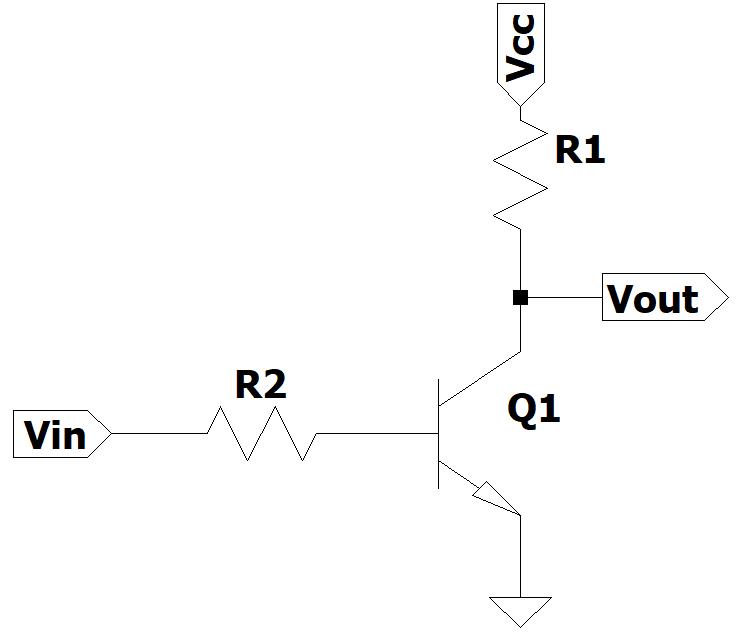
\includegraphics[scale = 0.45]{figs/ej1/not_rtl.png}
    \caption{Compuerta NOT con tecnolog\'ia RTL.}
\label{fig:ej1_rtl}
\end{figure}
\noindent
El funcionamiento de esta tecnolog\'ia se basa en que Vcc, la alimentaci\'on, se mantiene con una tensi\'on constante, por ejemplo 5V, mientras que en la entrada la tensi\'on puede variar. Si la tensi'on en la base del transistor representa un '0' l\'ogico, el transistor no conduce y por lo tanto, a la salida habr\'a un '1' l\'ogico. Por el otro lado, si se aplica un '1' l\'ogico en la base del transistor, comienza a conducir y la tensi\'on entre el colector y el emisor ser\'a de aproximadamente 0.3V representando un '0' l\'ogico.

\vspace{10mm}


{\large\textbf{Tecnolog\'ia TTL}}
\noindent
La compuerta NOT mediante tecnolog\'ia ttl funciona de la siguiente manera:

\begin{figure}[H]
\center
    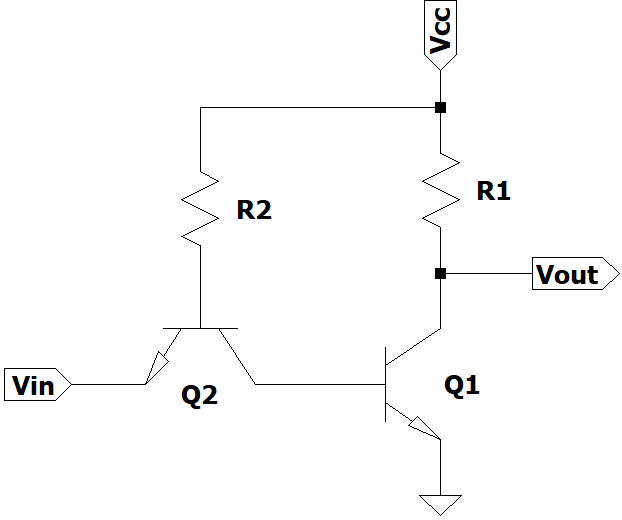
\includegraphics[scale = 0.55]{figs/ej1/not_ttl.png}
    \caption{Compuerta NOT con tecnolog\'ia TTL.}
\label{fig:ej1_ttl}
\end{figure}

\noindent\newline
El transistor Q2 trabaja tanto en directa como en inversa para dirigir la corriente hacia la base o desde la base del transistor Q1. Por lo tanto, si hay un '0' l\'ogico a la entrada Vin, con la alimentaci\'on en 5V, el transistor Q2 funciona en directa y la corriente es saliente de la base de Q1, por lo tanto, el transistor Q1 no conduce y hay un '1' a la salida. Por el contrario, si a la entrada hay un '1', el transistor Q2 est\'a polarizado en inversa y la corriente entra a la base de Q1 por lo que comienza a conducir y se ve un '0' a la salida.

\vspace{10mm}


{\large\textbf{Tecnolog\'ia MOS}}
\noindent

\begin{figure}[H]
\center
    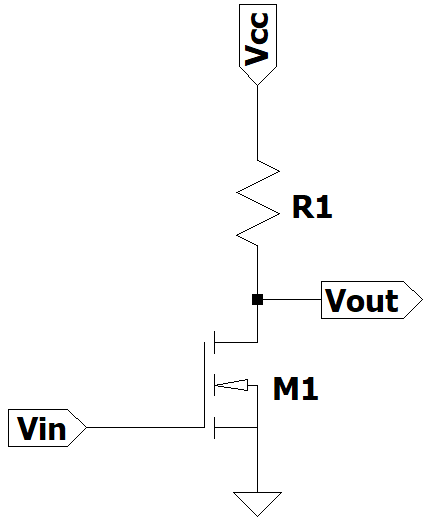
\includegraphics[scale = 0.55]{figs/ej1/not_mos.png}
    \caption{Compuerta NOT con tecnolog\'ia MOS.}
\label{fig:ej1_mos}
\end{figure}
\noindent

Se puede notar que el circuito es muy similar al rtl analizado previamente pero con un NMOS en lugar de BJT y sin la resistencia de base ya que en un MOS no circula corriente por ah\'i. Nuevamente con la tensi\'on de alimentaci\'on en 5V se analiza que pasa al aplicar a la entrada un '1' o un '0'. Si se inserta un '1', el transistor comienza a conducir y la tensi\'on entre base y emisor es de 5V por lo tanto a la salida se ve un '0'. Al insertar a la entrada un '0', el transistor no conduce y a la salida se ve un '1'.

\subsection{Mediciones}

Las mediciones se realizaron sobre un PCB que contiene las 3 compuertas juntas, como puede verse en la secci\'on \ref{ej1_pcb}.\newline
Se aliment\'o el circuito con una tensi\'on de 5V y luego, para realizar las distintas mediciones se le aplic\'o a la entrada de circuito una se\~nal cuadrada de 5V con nivel bajo en 0V para medir todo lo que est\'a relacionado con tiempos y una sen\~al tri\'angular para medir las tensi\'ones m\'inimas y m\'aximas como se detalla a continuaci\'on:\newline

\begin{itemize}
    \item VIH (\textit{High-level input voltage}): Es la m\'axima tensi\'on de entrada que el circuito interpreta como '0', produciendo un '1' a la salida. Se mide como el punto en donde la pendiente de $V_{in}(V_{out}) = -1$.
    \item VIL (\textit{Low-level input voltage}): Es la m\'inima tensi\'on de entrada que el circuito interpreta como '1', produciendo un '0' a la salida. Es el otro punto en el cual la pendiente es -1.
    \item VOH (\textit{High-level output voltage}): Es la m\'inima tensi\'on de salida con la cual hay un '1' a la salida.
    \item VOL (\textit{Low-level output voltage}): Es la m\'inima tensi\'on de salida con la cual hay un '0' a la salida.
    \item \textit{Noise margin}: Es la capacidad del circuito de tolerar ruido sin afectar el funcionamiento del mismo. Se clasifica en dos tipos:
    \begin{itemize}
        \item $NM_L$ (\textit{Low noise margin}): La diferencia entre VIL y VOL.
        \item $NM_H$ (\textit{High noise margin}): La diferencia entre VOH y VIH.
    \end{itemize}
    \item \textit{Propagation delay}: Tiempo desde que la se\~nal de entrada llega al 50\% hasta que la salida llega al mismo nivel.
    \item \textit{Transition time}: Tiempo que tarda la se\~nal de salida en llegar del 10\% hasta el 90\% de la tensi\'on al ir de '0' a '1' y viceversa para '1' a '0'.
    \item \textit{Maximum output current}: Debido a que la carga es un capacitor, se calcula como $I_c = C * \frac{dV_c}{dt}$ en donde la derivada se obtiene mediante la funci\'on \textit{math} del osciloscopio.
\end{itemize}

\begin{table}[H]
\center

\begin{tabular}{|l|c|c|c|}
\hline
\multicolumn{4}{|c|}{\textit{\textbf{Sin carga}}}                                                             \\ \hline
\multicolumn{1}{|c|}{\textbf{Tecnolog\'ia}} & \textbf{RTL} & \textbf{TTL} & \multicolumn{1}{l|}{\textbf{N-MOS}} \\ \hline
High-level input voltage.                 & 0.984V       & 0.7V         & 2.1V                                \\ \hline
Low-level input voltage.                  & 0.521V       & 0.338V       & 1.65V                               \\ \hline
High-level output voltage.                & 4.92V        & 4.998V       & 4.91V                                \\ \hline
Low-level output voltage.                 & 0.179V       & 0.096V       & 0.11V                               \\ \hline
Noise margin high.                        & 3.936V       & 4.298V       & 2.81V                               \\ \hline
Noise margin low.                         & 0.342V       & 0.242V       & 1.54V                               \\ \hline
Propagation delay high to low.            & 880ns        & 349ns        & 501ns                              \\ \hline
Propagation delay low to high.            & 29ns         & \#\#\#       & 23.95ns                              \\ \hline
Transition time high to low.              & 30.1ns       & \#\#\#         & 623ns                               \\ \hline
Transition time low to high.              & 680ns        & 382ns        & 714ns                                \\ \hline
\end{tabular}
\caption{Tabla de valores medidos sin carga.}
\label{tab:ej1_sin_carga}
\end{table}


\begin{table}[H]
\center
\begin{tabular}{|l|c|c|c|}
\hline
\multicolumn{4}{|c|}{\textit{\textbf{Con carga}}}                                                                                      \\ \hline
\multicolumn{1}{|c|}{\textbf{Tecnología}} & \textbf{RTL}              & \textbf{TTL}             & \multicolumn{1}{l|}{\textbf{N-MOS}} \\ \hline
High-level input voltage.                 & 1.02V                     & 0.822V                   & 2.15V                                \\ \hline
Low-level input voltage.                  & 0.543V                    & 0.315V                   & 1.59V                               \\ \hline
High-level output voltage.                & 4.87V                     & 4.99V                    & 4.9V                                \\ \hline
Low-level output voltage.                 & 0.247V                    & 0.067V                   & 0.18V                               \\ \hline
Noise margin high.                        & 3.85V                     & 4.168V                   & 2.75V                               \\ \hline
Noise margin low.                         & 0.296V                    & 0.248V                   & 1.41V                               \\ \hline
Propagation delay high to low.            & 8.25$\mu s$               & 7.7$\mu s$               & 6.2$\mu s$                             \\ \hline
Propagation delay low to high.            & 205$ns$                   & 46.8$ns$                 & 135$ns$                              \\ \hline
Transition time high to low.              & 146$ns$                   & 71$ns$                   & 1.12$\mu s$                               \\ \hline
Transition Time low to high.              & 25.7$\mu s$               & 21.1$\mu s$              & 23$\mu s$                                \\ \hline
Maximum output current.                   & \multicolumn{1}{l|}{11$mA$} & \multicolumn{1}{l|}{3$mA$} & \multicolumn{1}{l|}{28.2$mA$}         \\ \hline
\end{tabular}
\caption{Tabla de valores medidos con carga.}
\label{tab:ej1_con_carga}
\end{table}
\noindent
'\#\#\#' significa que dicho valor no pudo ser medido debido a las limitaciones del osciloscopio (\textit{Time rise} m\'inimo de 13ns).
\noindent\newline
\vspace{5mm}
\newline
En primer lugar, se puede observar de las mediciones hechas que el hecho de que el circuito tenga la carga de 1nF o que no lo tenga casi no afecta las tensiones de entrada ni las de salida. Mientras que por otro lado, produce que todos los tiempos, tanto de propagaci\'on como de transici\'on, aumenten, es decir, los circuitos son mas lentos con carga. \newline
Luego, se puede notar que la tecnolog\'ia TTL es la m\'as r\'apida en todos los tiempos, entre RTL y MOS, RTL es mas r\'apida en los tiempos de transici\'on pero es mas lenta en los de propagaci\'on. La gran ventaja de la tecnolog\'ia RTL es el hecho de que utiliza menos transistores que TTL. Finalmente, se puede observar que la compuerta NOT con MOS es la que presenta una mayor corriente de salida, por lo tanto es la que tiene mayor \textit{fanout}.

\subsection{Circuito utilizado}
\label{ej1_pcb}
\begin{figure}[H]
\center
    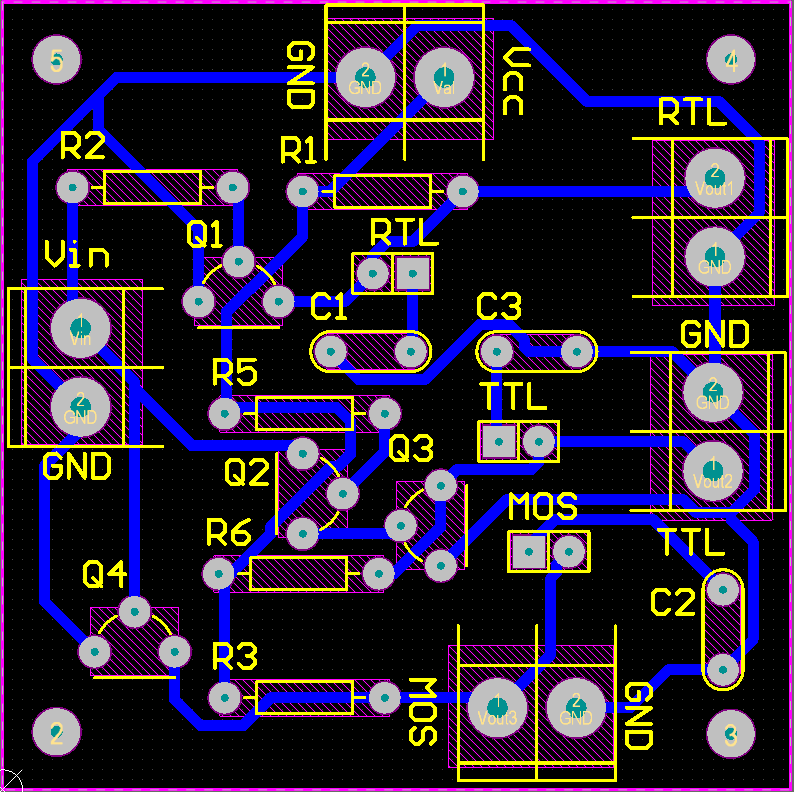
\includegraphics[scale = 0.55]{figs/ej1/ej1_PCB.png}
    \caption{Implementaci\'on del circuito en PCB.}
\label{fig:ej1_pcb}
\end{figure}
\noindent\newline
\newpage
\section{Ejercicio 2}
\subsection{Introducci\'on}
En el siguiente apartado se busca analizar la compatibilidad entre compuertas NOR de tecnolog\'ia TTL y CMOS. Para su comparaci\'on se utilizar\'an los integrados 74HC02, 74HCT02 y 74LS02.
\subsection{An\'alisis de datasheet}
Para realizar la comparaci\'on se tomaron los valores de tensiones de entrada y salida para los estados 1 y 0 de las diferentes compuestas, especificados en las hojas de datos (74HC02 \footnote{http://www.ti.com/lit/ds/symlink/sn74hc02.pdf}, 74HCT02\footnote{http://www.ti.com/lit/ds/symlink/sn74hct02.pdf}
y 74LS02\footnote{http://www.ti.com/lit/ds/sdls027/sdls027.pdf}).
\begin{table}[H]
\centering
\begin{tabular}{|c||c|c|c|}
\hline
    & 74HC02 & 74HCT02 & 74LS02 \\ \hline \hline 
$V_{ih}[V]$ & 3,15   & 2       & 2      \\
$V_{oh}[V]$ & 4,4    & 4,4     & 2,4    \\
$V_{il}[V]$ & 1,35   & 0,8     & 0,8    \\
$V_{ol}[V]$ & 0,26   & 0,26    & 0,4    \\ \hline
\end{tabular}
\caption{Margenes de ruido, compuertas NOR}
\label{ej2_table_nor}
\end{table}
Para garantizar la compatibilidad entre dos compuertas se debe cumplir, inicialmente, que $V_{ih} > V_{oh}$ y  $V_{il} < V_{ol}$, observando la tabla \ref{ej2_table_nor} se puede apreciar que en la \'unica combinaci\'on de compuertas que no se cumple esta condici\'on es al cargar una compuerta 74LS02 con una compuerta 74HC02, es decir cargando una compuerta de tecnolog\'ia TTL con una de tecnolog\'ia CMOS que no se encuentre adaptada para tal utilidad, ya que para la compuerta 74HC02 la tensi\'on m\'inima de entrada ($V_{ih}$) para un 1 l\'ogico es de 3.15V lo cual es superior a la tensi\'on de salida m\'ininma ($V_{oh}$) para un 1 l\'ogico del integrado 74LS02.
\subsection{Medici\'on}
Conectando ambas compuertas en cascada y con las entradas cortocircuitadas, para obtener dos compuertas NOT en casacada, se mide la salida de la primer compuerta y la salida de la segundo excitando al circuito con una rampa a fin de poder observar la respuesta en la transici\'on de estados del circuito.
\begin{figure}[H]
\begin{subfigure}{.5\textwidth}
  \centering
  % include first image
  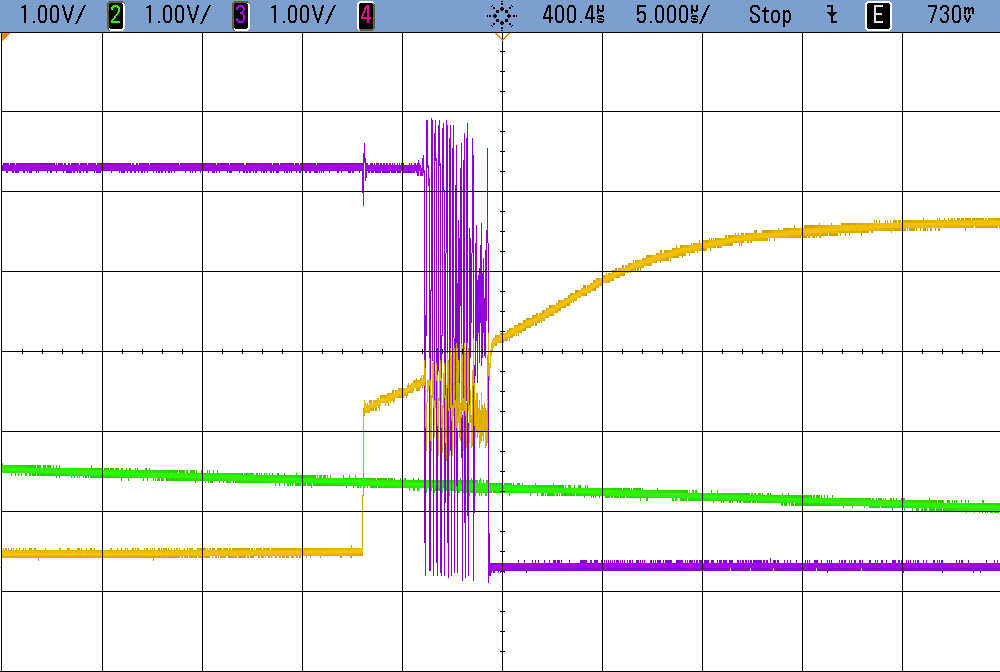
\includegraphics[width=.85\linewidth]{figs/EJ2/LS_HC_0_1.png}  
  \caption{Transici\'on 0-1 de LS.}
  \label{ej2_fig:LS_HC_01}
\end{subfigure}
\begin{subfigure}{.5\textwidth}
  \centering
  % include second image
  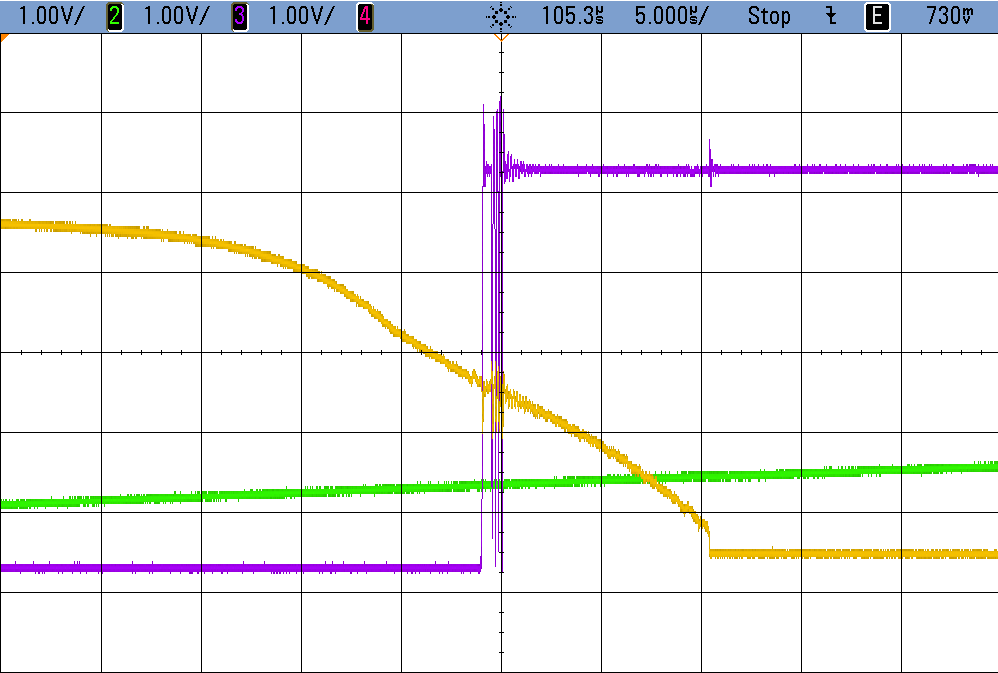
\includegraphics[width=.85\linewidth]{figs/EJ2/LS_HC_1_0.png}  
  \caption{Transici\'on 1-0 de LS.}
  \label{ej2_fig:LS_HC_01}
\end{subfigure}
\caption{Respuesta HC cargando LS.}
\label{ej2_fig:LS_HC}
\end{figure}

\begin{figure}[H]
\begin{subfigure}{.5\textwidth}
  \centering
  % include first image
  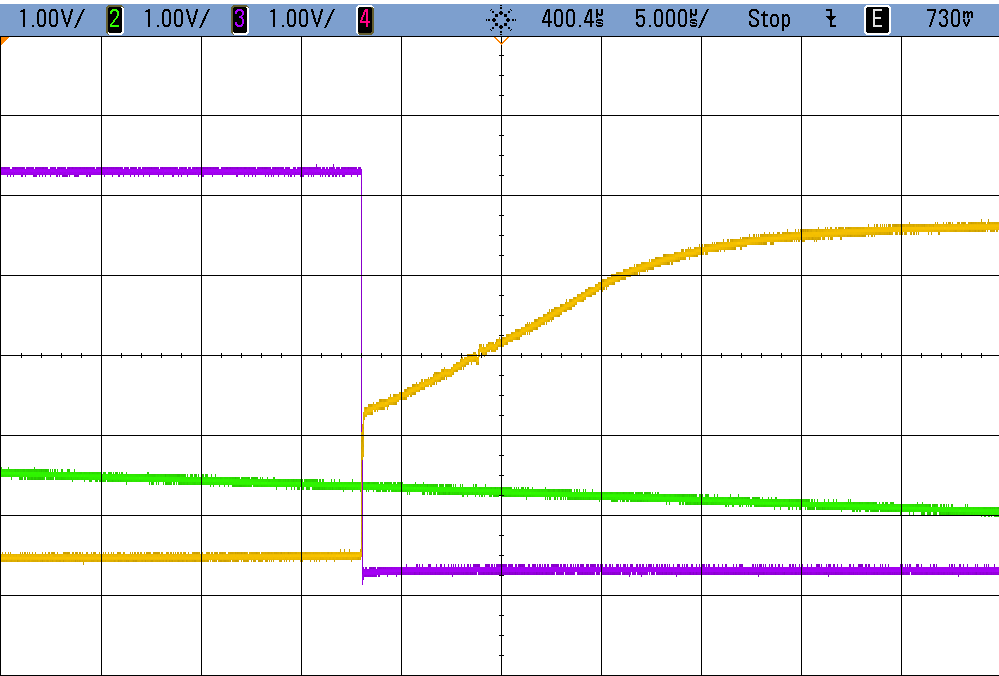
\includegraphics[width=.8\linewidth]{figs/EJ2/LS_HCT_0_1.png}  
  \caption{Transici\'on 0-1 de LS.}
  \label{ej2_fig:LS_HCT_01}
\end{subfigure}
\begin{subfigure}{.5\textwidth}
  \centering
  % include second image
  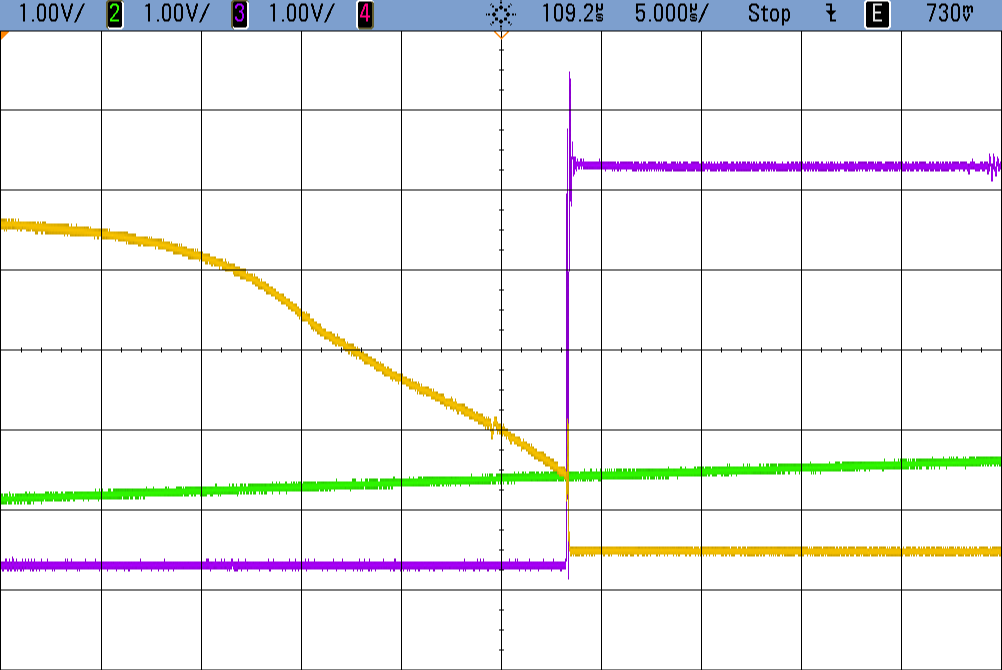
\includegraphics[width=.8\linewidth]{figs/EJ2/LS_HCT_1_0.png}  
  \caption{Transici\'on 1-0 de LS.}
  \label{ej2_fig:LS_HCT_01}
\end{subfigure}
\caption{Respuesta HCT cargando LS.}
\label{ej2_fig:LS_HCT}
\end{figure}

De esta forma se puede ver que al cargar la compuerta LS con la compuerta HC, se presentan oscilaciones debido a la indeterminacion del estado en la compuerta HC, este inconveniete es solucionado en las compuertas de la familia HCT las cuales estan diseñadas para garantizar la compatibilidad con las compuertas de tecnologia TTL que presentan diferentes niveles de ruido.\\
\subsection{Fanout}
Otro aspecto para analizar en la compatibilidad de compuertas es la capacidad de una compuerta de suministrar la corriente que le demanda la carga, ya que de no poder suministrarla adecuadamente, a la salida puede ser malinterpretado el estado l\'ogico.\\
Las compuertas HC02 y HCT02 al pertenecer a la familia de compuertas CMOS demandan corrientes de entrada muy pequeñas, seg\'un las hojas de datos 100nA, lo cual favorece la conexi\'on de estas compuertas como carga de otras compuertas.


\newpage
\section{Ejercicio 3}
\subsection{Introducci\'on}
\noindent
En este ejercicio se plantea la implementaci\'on de la tabla de verdad propuesta por la consigna, la misma se puede ver en la tabla \ref{ej3_tabla_de_verdad}. Para ello se hará uso de compuertas lógicas de tecnología CMOS dispuestas en una placa PCB, con la intención de realizar mediciones relevantes de la configuración de menor costo, con la finalidad de proponer cambios de ser necesarios para evitar posibles problemas con dicha implementación. 
%
\subsection{An\'alisis Te\'orico}
\noindent
De esta manera se hallar\'a el circuito que se realizar\'a mediante las simplificaciones del diagrama de Karnaugh haciendo uso de la tabla propuesta. De esta manera en la imagen siguiente se procede a mostrar dicho diagrama seleccionando los grupos de inter\'es que generan la configuraci\'on de menor costo.
%
\begin{table}[H]
\caption{Tabla propuesta}
\label{ej3_tabla_de_verdad}
\centering
\begin{tabular}{|l|l|l||l|}
\hline
A & B & C & Y \\ \hline \hline
0 & 0 & 0 & 0 \\ \hline
0 & 0 & 1 & 1 \\ \hline
0 & 1 & 0 & 1 \\ \hline
0 & 1 & 1 & 1 \\ \hline
1 & 0 & 0 & 0 \\ \hline
1 & 0 & 1 & 1 \\ \hline
1 & 1 & 0 & 0 \\ \hline
1 & 1 & 1 & 0 \\ \hline
\end{tabular}
\end{table}
%
\begin{center}
    \begin{Karnaughvuit}
       \minterms{1,4,5,6}
        \maxterms{0,2,3,7}
       %\indeterminats{2,5}
       \implicantcostats{4}{6}{green}
       \implicant{1}{5}{blue}
    \end{Karnaughvuit}
\end{center}
%
%
%
\noindent
Así la configuraci\'on l\'ogica que cumple este circuito es la de la ecuaci\'on \ref{ej3_eq1}.
%
\begin{equation}
    \overline{A} \cdot B+\overline{B} \cdot C
    \label{ej3_eq1}
\end{equation}
%
\noindent
Dicha ecuación representa la configuración lógica de menor costo que cumple con la tabla propuesta (tabla \ref{ej3_tabla_de_verdad}).\\
\noindent
De esta forma el circuito que cumple con dicha ecuación se muestra en la figura \ref{ej3_circuito}.
%
\begin{figure}[H]
    \centering
        \centering
        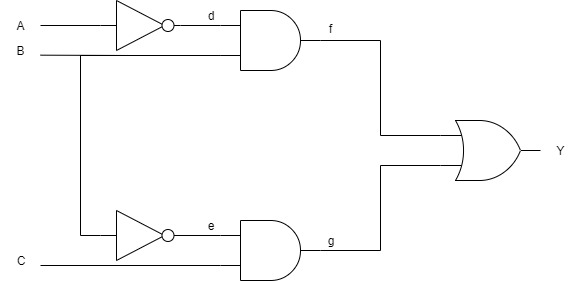
\includegraphics[width=0.8\textwidth]{figs/Ej3/circuito1.jpg} % first figure itself
         \caption{Figura del circuito con la configuraci\'on de menor costo}
         \label{ej3_circuito}
\end{figure}
%
\noindent
El problema con este circuito es que puede presentar glitches, los mismos pueden ser percibidos en el diagrama de Karnaugh debido a la existencia de 2 unos adyacentes que no tienen un grupo que los conecte entre sí, de esta manera el sistema puede pasar por un cero momentáneamente aun cuando la salida se mantenga en 1, esto es lo que en inglés se denominan static Hazards.\\
\noindent
Esto también se puede apreciar mejor al realizar el diagrama temporal del circuito, que se muestra a continuación en la figura \ref{ej3_glitch}, en donde por simplicidad se presupone que las compuertas utilizadas presentan el mismo retraso temporal.
%
\begin{figure}[H]
    \centering
        \centering
        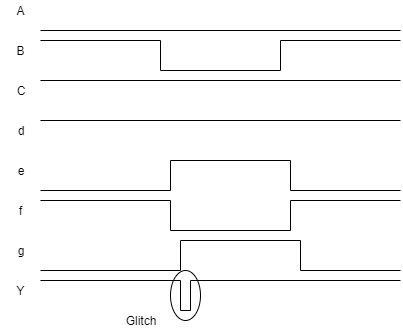
\includegraphics[width=0.6\textwidth]{figs/Ej3/glitch.jpg} % first figure itself
         \caption{Diagramas temporales del circuito en donde se aprecia el glitch en la salida.}
         \label{ej3_glitch}
\end{figure}
%
\noindent
Este glitch (indeseado) es provocado debido a los diferentes tiempos de propagaci\'on de las compuertas utilizadas, es decir existe un camino que presenta m\'as compuertas l\'ogicas que el otro por lo que se genera un momento en donde en la entrada de la compuerta or a la salida se tienen 2 ceros que no se deber\'ian encontrar, esto hace que a la salida se observe un cero por un breve instante de tiempo (el tiempo de propagación de la compuerta tomado).\\
Para evitar este tipo de glitch, lo que se hace es realizar una configuración de mayor costo, es decir, considerar un grupo extra (y por consiguiente mayor cantidad de compuertas l\'ogicas en el diseño total) que abarque los 2 unos que se hallaban adyacentes sin estar conectados mediante un grupo. Esto se puede ver en el diagrama de Karnaugh siguiente.
%
\begin{center}
    \begin{Karnaughvuit}
       \minterms{1,4,5,6}
        \maxterms{0,2,3,7}
       %\indeterminats{2,5}
       \implicantcostats{4}{6}{green}
       \implicant{1}{5}{blue}
       \implicant{4}{5}{red}
    \end{Karnaughvuit}
\end{center}
%
\noindent
De esta forma la configuraci\'on l\'ogica que cumple este circuito es la de la ecuaci\'on \ref{ej3_eq2}.
%
\begin{equation}
    \overline{A} \cdot B+\overline{B} \cdot C+\overline{A} \cdot C
    \label{ej3_eq2}
\end{equation}
%
\noindent
Por ello el circuito que cumple con dicha ecuación se muestra en la figura \ref{ej3_circuito2}.
%
\begin{figure}[H]
    \centering
        \centering
        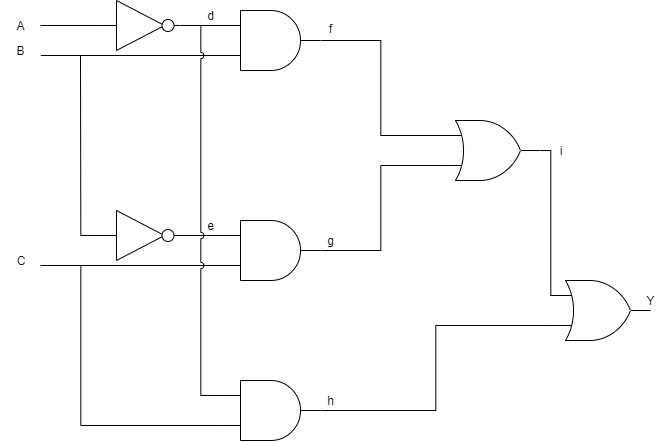
\includegraphics[width=0.6\textwidth]{figs/Ej3/circuito2.jpg} % first figure itself
         \caption{Circuito con la corrección para evitar glitches}
         \label{ej3_circuito2}
\end{figure}
%
%
\subsection{Implementaci\'on}
%
\noindent
Para comprobar esto, se realiz\'o en PCB un diseño en donde se puede trabajar tanto con un circuito como con otro a la vez, esto permite observar las diferentes salidas de cada uno para con ello poder contrastarlas y hallar diferencias entre los métodos trabajados.\\
\noindent
De esta forma, la placa PCB utilizada se puede observar en la imagen \ref{ej3_placa}.
Para la misma se utilizaron los integrados 74HC08 para las compuertas and, 74HC04 para las compuertas not y 74HC32 para las compuertas or. Los tiempos de propagación de dichas compuertas se muestran a continuación en la tabla \ref{tabla_comp_tiempos_prop}, y se pueden ver en en las hojas del fabricante \href{ http://www.ti.com/lit/ds/symlink/sn74hc08.pdf}{74HC08}, \href{http://www.ti.com/lit/ds/symlink/sn74hc04.pdf}{74HC04}, \href{http://www.ti.com/lit/ds/symlink/sn74hc32.pdf}{74HC32}.
%
\begin{table}[H]
\caption{Tabla con los tiempos de propagación de las compuertas utilizadas.}
\label{tabla_comp_tiempos_prop}
\centering
\begin{tabular}{|l||l|l|}
\hline
integrado & normal (ns) & maximo (ns) \\ \hline \hline
74HC04    & 9      & 22     \\ \hline
74HC08    & 10     & 20     \\ \hline
74HC32    & 12     & 18     \\ \hline
\end{tabular}
\end{table}
%
%
%
\begin{figure}[H]
    \centering
        \centering
        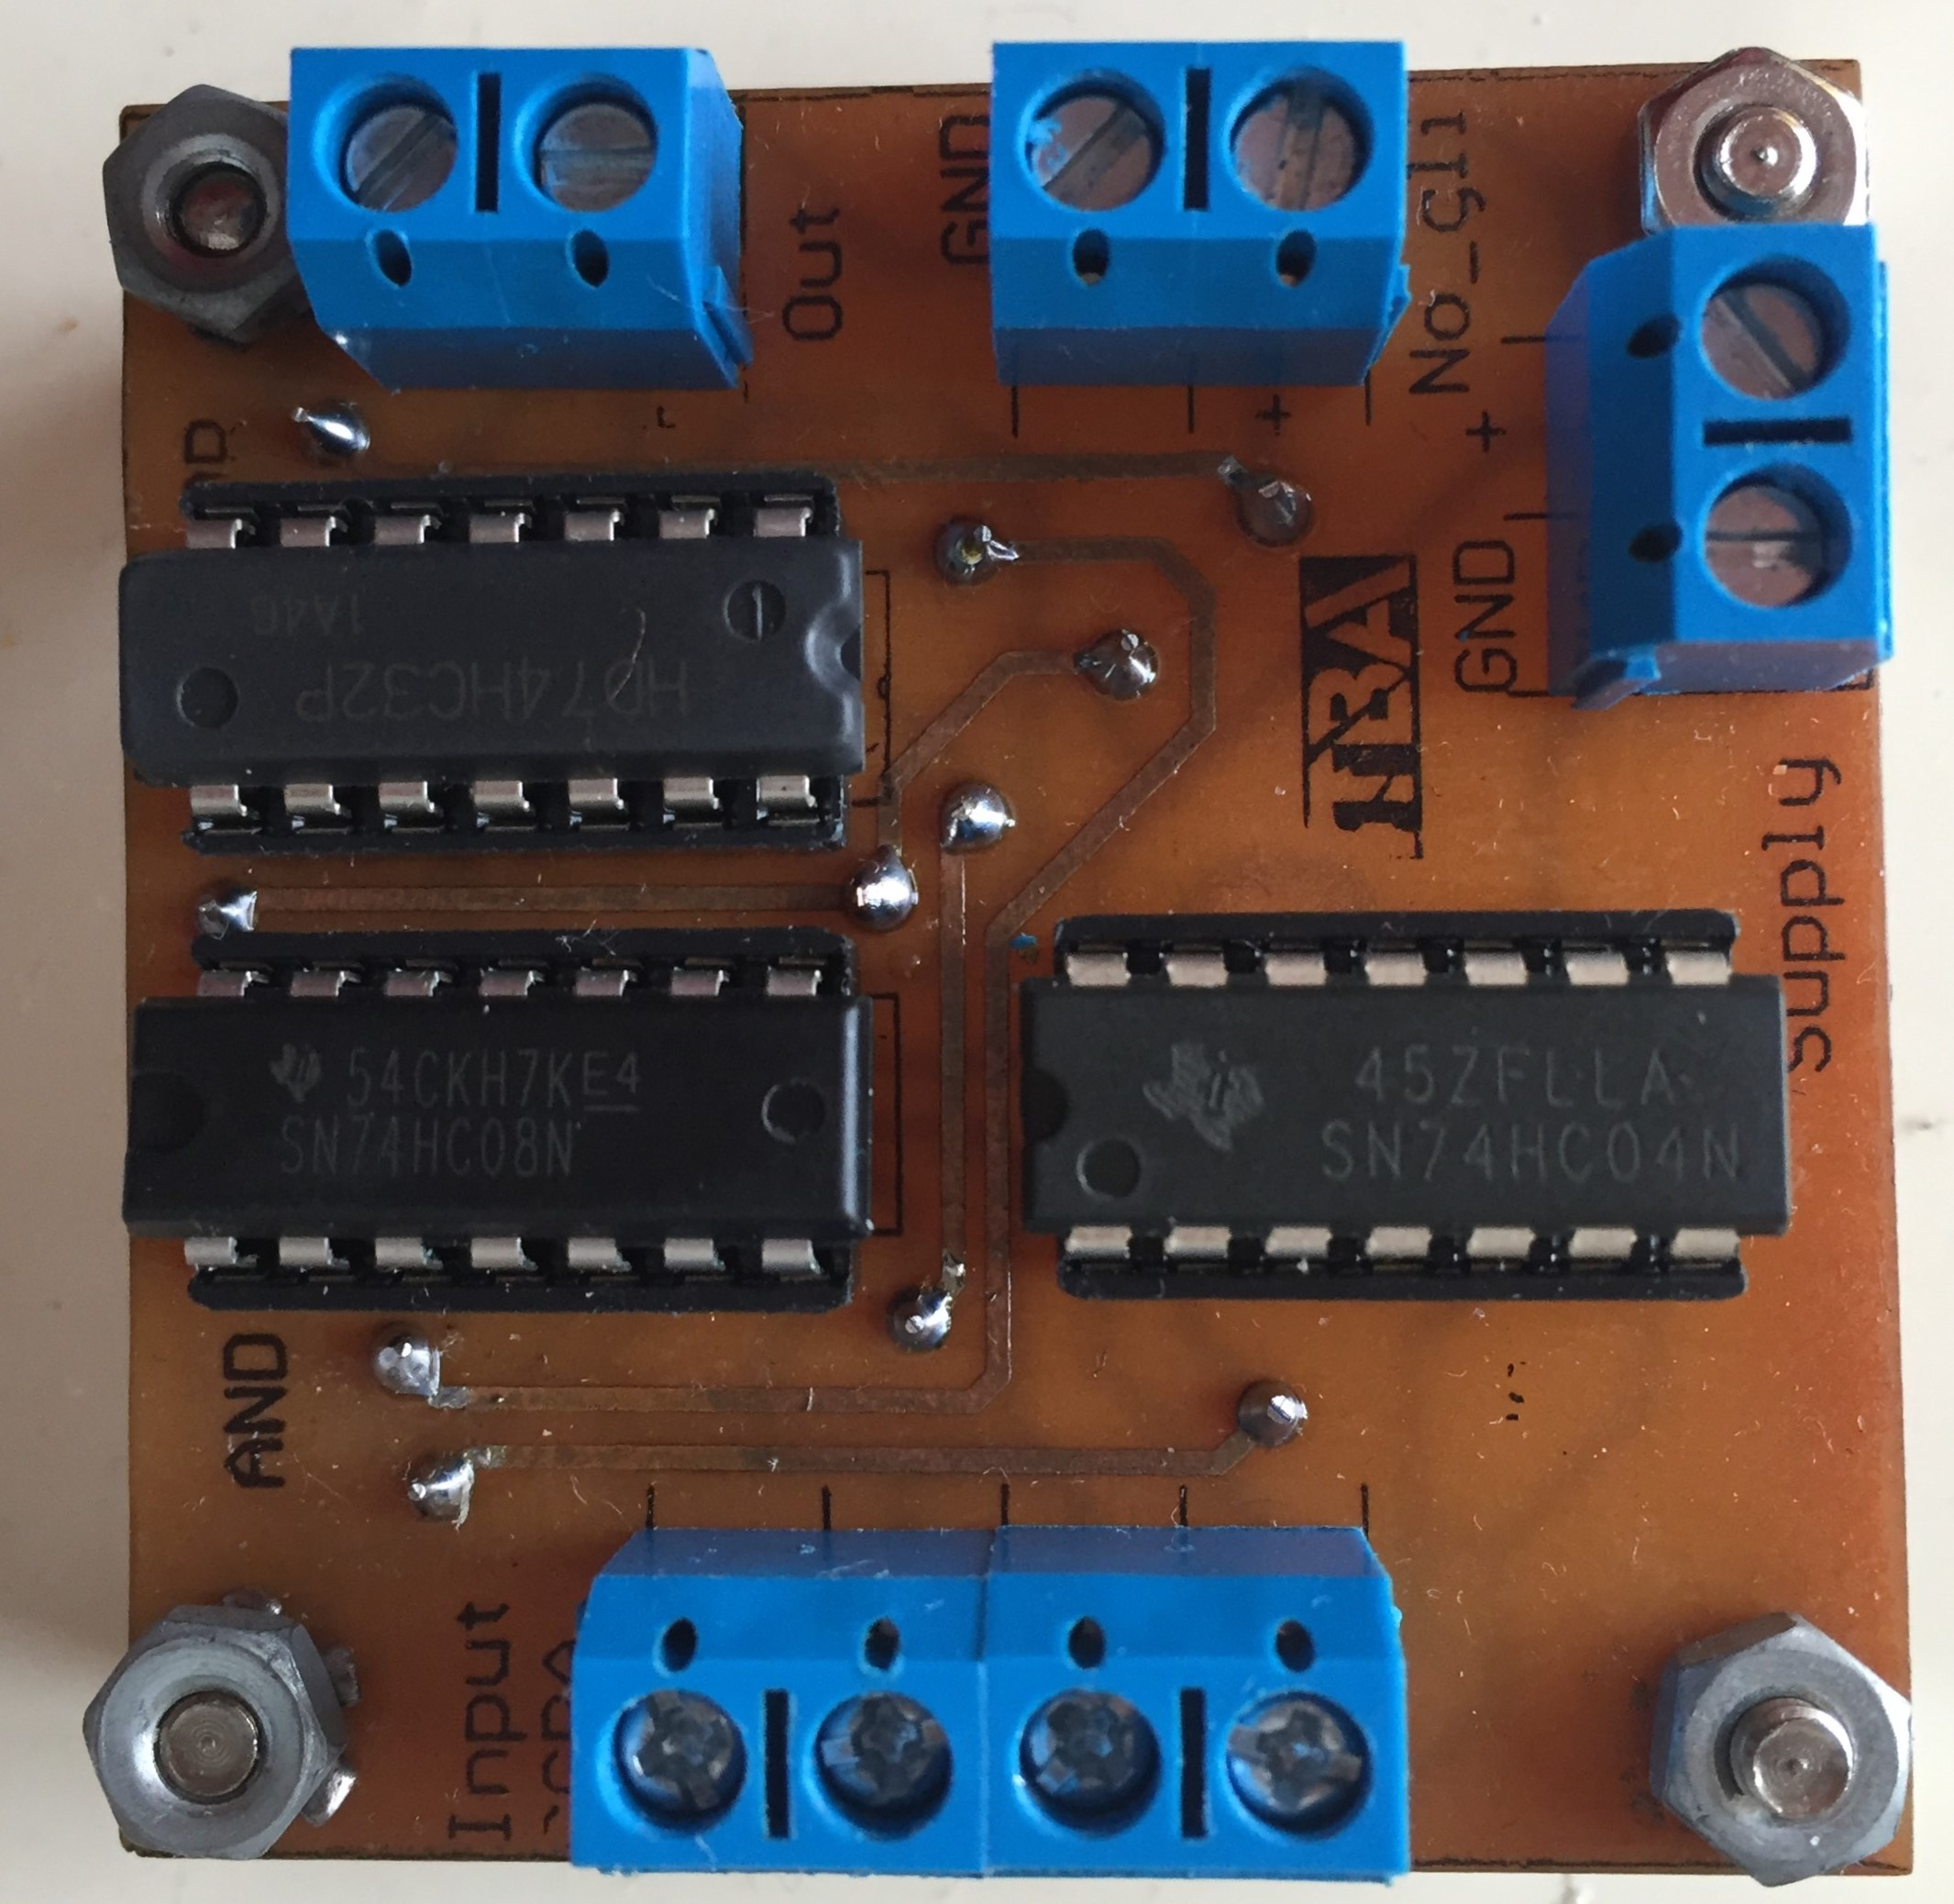
\includegraphics[width=0.6\textwidth]{figs/Ej3/Circuito_PCB.jpg} % first figure itself
         \caption{placa PCB utilizada}
         \label{ej3_placa}
\end{figure}
%
\subsection{Mediciones y Conclusiones}
\noindent
A continuación en la figura \ref{ej3_medicion} se muestra la medición del circuito a la salida del mismo, donde se superponen la salida del circuito con la configuración de menor costo y la salida del circuito con la configuración de mayor costo que soluciona el problema de los glitches, las mismas se realizaron en simultaneo en las 2 salidas del circuito destinadas a este fin, al pasar de la configuración abc=001 a abc=011, para el cambio de B se utilizó un generador de onda cuadrada con tensiones de 0V mínima y 5V máxima.\\ Cabe destacar que para poder observar el glitch es muy importante utilizar puntas x10 ya que la capacidad de las puntas x1 impide la correcta visualización de la caída en tensión.
%
\begin{figure}[H]
    \centering
        \centering
        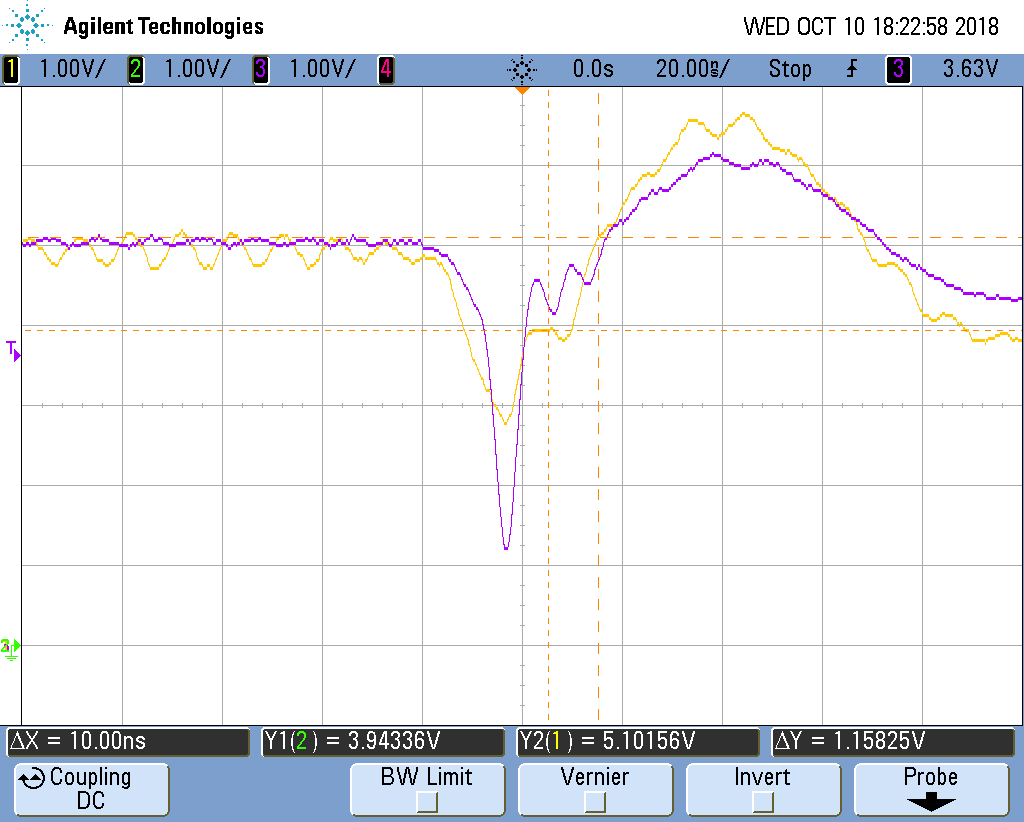
\includegraphics[width=0.6\textwidth]{figs/Ej3/x10_se_ve_glitchesito_ojo_limit_oscil.png} % first figure itself
         \caption{Medición realizada donde se aprecia el glitch a la salida.}
         \label{ej3_medicion}
\end{figure}
%
\noindent
En la imagen \ref{ej3_medicion} podemos ver las 2 salidas deseadas, la salida sin la corrección es la de color violeta, y la salida corregida corresponde a la linea de color amarillo.\\
En el osciloscopio se observa como el valor de la salida violeta cae por debajo del límite inferior tomado como High por las compuertas con tecnología CMOS (imagen \ref{ej3_cmos}), pasa por la zona de transición y llega a ser inferior que el límite superior de lo que se considera como LOW, es decir un cero lógico durante un tiempo comparable con el de las compuertas utilizadas, llegando a valer 1,2 V. Esto tiene sentido si se observa el diagrama temporal analizado anteriormente donde el tiempo del glitch se correspondía con el tiempo de propagación tomado para las compuertas. Mientras que la salida amarilla correspondiente a la salida del sistema con el glitch corregido presenta una desviación mucho menor que le permite nunca bajar lo suficiente para ser considerado por la compuerta como un 0 lógico, vemos por tanto que en la salida corregida no existe glitch mientras que en la salida violeta es decir la de menor costo si lo hay.
%
\begin{figure}[H]
    \centering
        \centering
        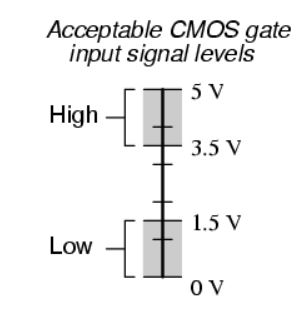
\includegraphics[width=0.4\textwidth]{figs/Ej3/cmosvoltages.JPG} % first figure itself
         \caption{Tensiones de entrada consideradas como HIGH y LOW en una compuerta con tecnología CMOS}
         \label{ej3_cmos}
\end{figure}
\newpage
\section{Ejercicio 4}
\noindent
En la siguiente secci\'on se busca analizar los tiempos caracter\'isticos de la compuerta 74HC02, medidas con carga y sin carga. Adem\'as se analizar\'a la respuesta de la fuente de alimentaci\'on de las compuertas, trabajando en altas frecuencias.
\subsection{Desarrollo emp\'irico}
\noindent
Inicialmente se midi\'o la salida de la compuerta NOR, de tecnolog\'ia CMOS, con las entradas cortocircuitadas y sin carga, y luego con el circuito propuesto en la figura \ref{ej4_fig:circuito}, buscando medir el \textit{time rise}, el \textit{fall time} y el tiempo de propagaci\'on en la transici\'on del estado alto a bajo, y del estado bajo al alto.\\
\begin{figure}[H]
    \centering
    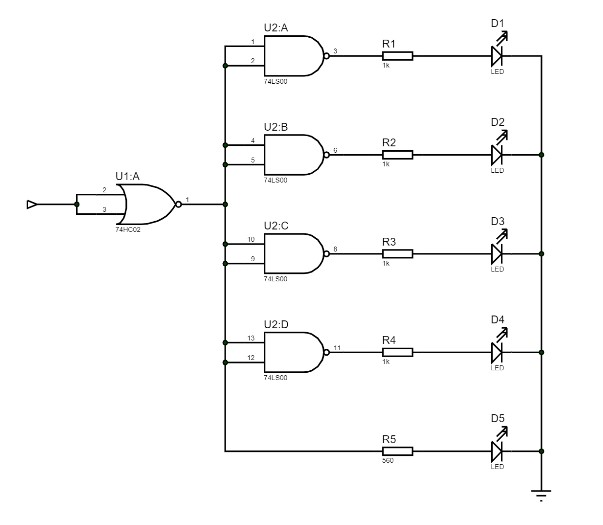
\includegraphics[width=0.5\linewidth]{figs/EJ4/esquematico.jpg}
    \caption{Circuito de medici\'on}
    \label{ej4_fig:circuito}
\end{figure}
Para los cuatro tiempos a medir se utilizaron los cursores del osciloscopio utilizando la funci\'on de \textit{tracking} como se ejemplifica en la figura \ref{ej4_fig:HC}.
\begin{figure}[H]
\begin{subfigure}{.5\textwidth}
  \centering
  % include first image
  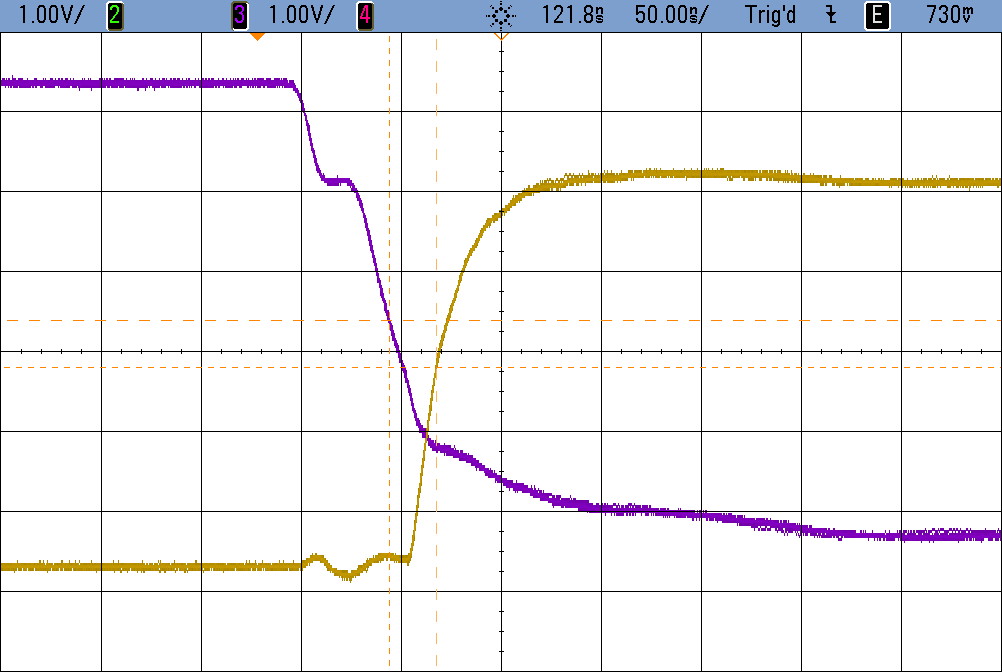
\includegraphics[width=.85\linewidth]{figs/EJ4/HC_Prop.png}  
  \caption{Medici\'on del tiempo de propagaci\'on.}
  \label{ej4_fig:HC_prop}
\end{subfigure}
\begin{subfigure}{.5\textwidth}
  \centering
  % include second image
  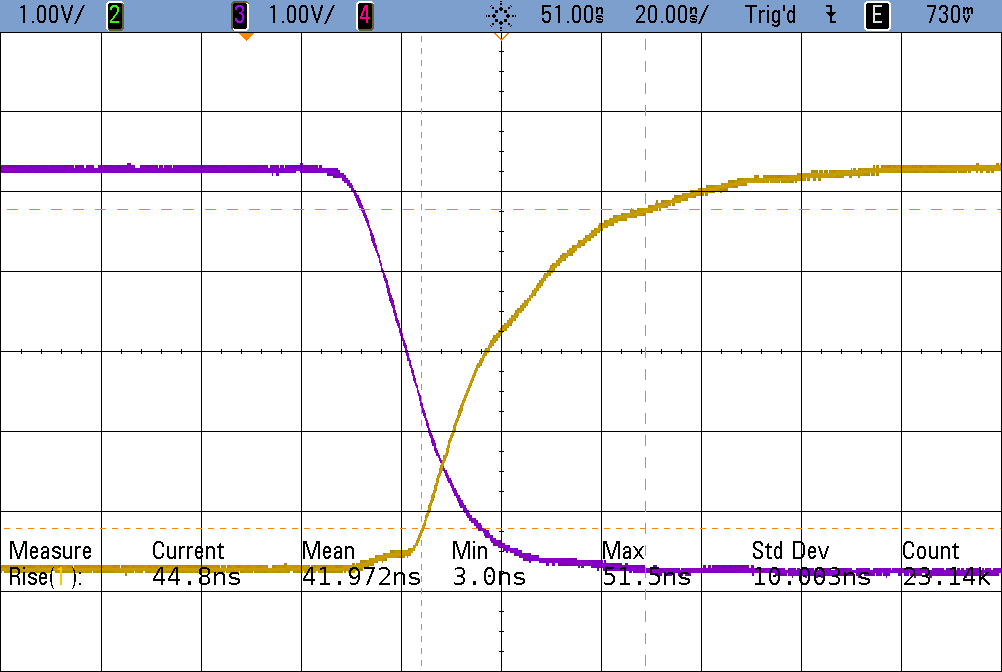
\includegraphics[width=.85\linewidth]{figs/EJ4/HC_TR.png}  
  \caption{Medici\'on del \textit{time rise}.}
  \label{ej4_fig:HC_rise}
\end{subfigure}
\caption{Mediciones sobre la compuerta, violeta-entrada, amarilla-salida}
\label{ej4_fig:HC}
\end{figure}
De estas mediciones se obtuvieron los resultados de la tabla \ref{ej4:table_times}, en todos los casos se puede apreciar que los tiempos con carga son mayores que sin carga, sin embargo dichas asimetr\'ias son despreciables y las mismas pueden ser explicadas debido a la demanda de corriente de la rama de $R_5$ y $D_5$. 
\begin{table}[H]
\centering
\begin{tabular}{|c||c|c|}
\hline
          & Sin carga & Con carga \\ \hline \hline
$t_r$     & 43       & 45       \\
$t_f$     & 44,5     & 48       \\
$t_{prop H-L}$ & 10,5     & 12      \\
$t_{prop L-H}$ & 13,5     & 15,5     \\ \hline
\end{tabular}
\caption{Mediciones de tiempos caracter\'isticos, en ns.}
\label{ej4:table_times}
\end{table}
\subsection{Medici\'on a altas frecuencias}
\noindent
Una vez medidos los tiempos caracter\'isticos, para continuar el an\'alisis se aumento la frecuencia del generador a 100KHz, y se midi\'o la alimentaci\'on de la compuerta 74HC02.\\
\begin{figure}[H]
\begin{subfigure}{.5\textwidth}
  \centering
  % include first image
  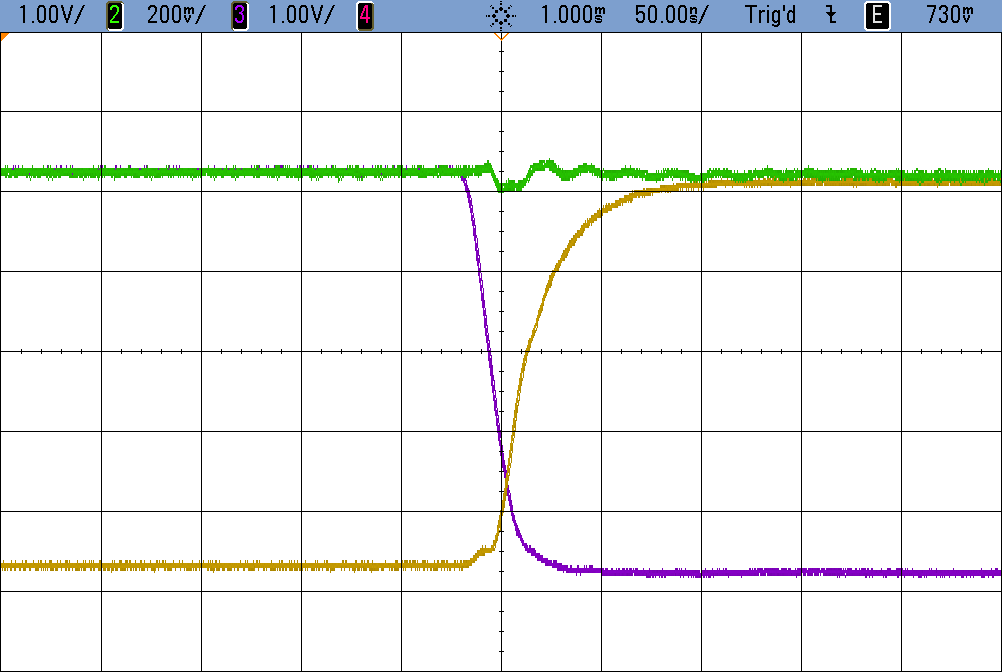
\includegraphics[width=.85\linewidth]{figs/EJ4/HF_sin_C.png}  
  \caption{Sin capacitor de desacople.}
  \label{ej4_fig:HF_sin_C}
\end{subfigure}
\begin{subfigure}{.5\textwidth}
  \centering
  % include second image
  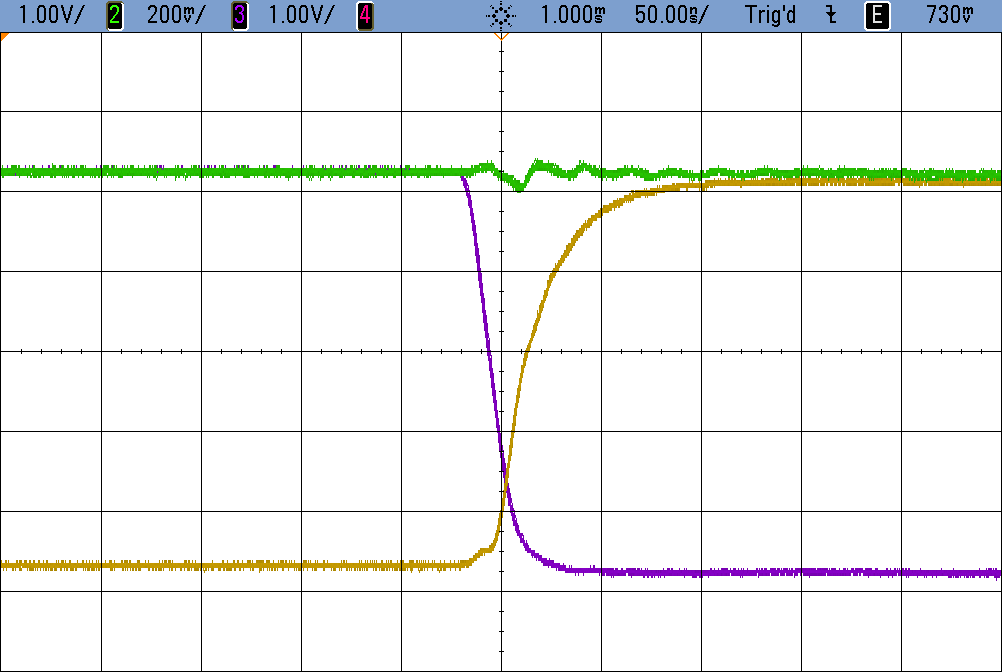
\includegraphics[width=.85\linewidth]{figs/EJ4/HF_con_C.png}  
  \caption{Con capacitor de desacople.}
  \label{ej4_fig:HF_con_C}
\end{subfigure}
\caption{Medici\'on de la alimentaci\'on (verde), salida (amarilla), entrada (violeta)}
\label{ej4_fig:HF}
\end{figure}
En la figura \ref{ej4_fig:HF_sin_C}, se puede apreciar que en la transici\'on de estados, en la alimetaci\'on se produce una respuesta subamortiguada, esto es debido a una mayor exigencia de corriente en dicho momento por parte del integrado.\\
Se intent\'o cambiar dicha respuesta con la inclusi\'on de un capacitor de desacople en los terminales de alimentaci\'on del integrado, el mismo seg\'un lo especificado en el libro de aplicac\'on  del fabricante\footnote{http://www.ti.com/lit/an/sdya002/sdya002.pdf} debe ser de 100nF. Agregando dicho capacitor al circuito se busc\'o reducir dicha respuesta subamortiguada, lo obtenido se muestra en la figura \ref{ej4_fig:HF_con_C}, en la que es posible observar que no se logr\'o corregir completamente el comportamiento indeseado de la fuente, sin embargo se redujo su duraci\'on levemente.\\
Al trabajarse con una sola de las compuertas las demandas de corriente al circuito de alimentaci\'on no fueron excesivas, pero si se hubiese trabajado con la totalidad de las compuertas integradas, el capacitor de desacople hubiese cumplido una funci\'on de mayor relevancia.
\subsection{Conclusiones}
\noindent
Midiendo los tiempos caracter\'isticos de la compuerta 74HC02 de tecnolog\'ia CMOS se pudo observar la influencia de la carga en los mismos, viendo que al aumentar los niveles de carga, aumentaban tanto el tiempo de propagaci\'on como el \textit{rise time} y el \textit{fall time}.\\
Adicionalmente fue posible observar que dependiendo las condiciones de trabajo puede ser necesaria la inclusi\'on de capacitores de desacople al utilizar integrados l\'ogicos, ya que la respuesta transitoria de la fuente de alimentaci\'on puede generar niveles de tensi\'on que se encuentren fuera del rango permitido por el fabricante. 
\newpage
\section{Ejercicio 5}
\subsection{Introducci\'on}
\noindent
En el presente apartado se estudiar\'a el comportamiento y compatibilidad de dos compuertas l\'ogicas. Se utilizar\'a para ello una compuerta AND de tecnolog\'ia TTL y una compuerta OR de tecnolog\'ia CMOS. Inicialmente se analizar\'an sus respuestas individualmente y luego, de la forma en que se aprecia en la figura \ref{ej5_fig:compuertasjuntas}, se unir\'an la entrada de la OR-CMOS con la salida de la AND-TTL. A partir de esto, se observar\'an los nuevos resultados y se investigar\'an los distintos problemas que se pudieran presentar junto a sus posibles soluciones.

\begin{figure}[H]
    \centering
    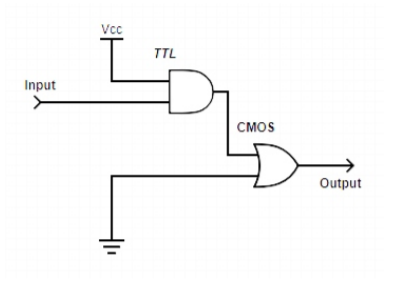
\includegraphics[scale=0.6]{figs/ej5/compuertas_juntas.png}
    \caption{Conexi\'on de las compuertas utilizadas.}
    \label{ej5_fig:compuertasjuntas}
\end{figure}

\subsection{An\'alisis previo}

\noindent
 Existen distintas consideraciones que deben realizarse cuando se interact\'ua entre las tecnolog\'ias a utilizar. En primer lugar, si se requiriera alimentar a integrados de ambas con una \'unica fuente, el rango posible de valores a utilizar se encuentra limitado por la tensi\'on aceptable de la tecnolog\'ia TTL, el cual se encuentra t\'ipicamente entre $4,75V$ y $5,25V$. 
 
\noindent
Luego, a modo de analizar la forma de realizar las correspondientes conexiones entre la salida de una tecnolog\'ia y la entrada de la otra, es necesario estudiar con que tensiones trabaja cada una en estos puntos. As\'i, en la figura \ref{ej5_fig:comparador_rangos} se detallan los valores alrededor de los cuales se encuentran los par\'ametros necesarios. Analizando lo que sucede al contar con una salida TTL y una entrada CMOS, se observa que $VOL_{TTL} < VIL_{CMOS}$ y que $VOH_{TTL} < VIH_{CMOS}$. Dado el primer caso (estado 0), no existen problemas por compatibilidad. No obtante, con respecto al segundo caso (estado 1), dado que la tensi\'on de salida en alto de una compuerta TTL puede ser menor que la tensi\'on en entrada en alto de una compuerta CMOS, \textbf{pueden presentarse problemas por incompatibilidad de tensi\'on}\label{ej5_ref:problema}.

\begin{figure}[H]
    \centering
    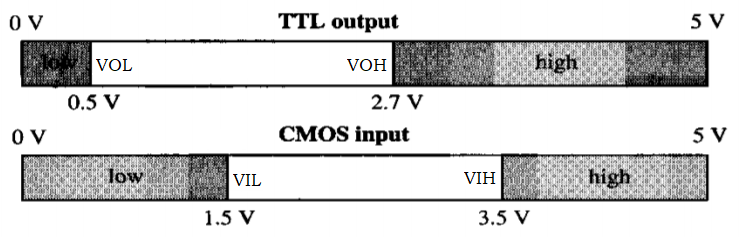
\includegraphics[scale=0.4]{figs/ej5/comparador_rangos_completo.png}
    \caption{Rangos de entrada y salida t\'ipicos de las tecnolog\'ias a utilizar.}
    \label{ej5_fig:comparador_rangos}
\end{figure}


\noindent
En adici\'on a la compatibilidad entre las tensiones, para la interconexi\'on de distintas tecnolog\'ias tambi\'en es necesario estudiar los requerimientos de corriente de cada una de ellas. Un factor de problem\'atica se da en el caso en que una compuerta de salida no pueda suministrar la corriente necesaria por la compuerta de entrada para interpretar un estado como tal. A partir de esto se detallan en la tabla \ref{ej5_tab:current_comparison} los valores de corriente con los que trabajan t\'ipicamente los integrados de tecnolog\'ia TTL y CMOS.

\begin{table}[H]
\centering
\begin{tabular}{ccc}
Par\'ametro & CMOS (74HC/HCT)     & TTL (74LS)   \\
IIH (min)      & $1\mu A$      & $20\mu A$  \\
IIL (min)      & $1\mu A$      & $0.6mA$ \\
IOH (m\'ax)      & $4mA$      & $0.4mA$ \\
IOL (m\'ax)      & $4mA$      & $8mA  $
\end{tabular}
\caption{Corrientes de entrada y salida de las tecnolog\'ias a utilizar.}
\label{ej5_tab:current_comparison}
\end{table}

\noindent
A partir de estas consideraciones, si se analiza la tabla \ref{ej5_tab:current_comparison} se concluye que \textbf{no existen problemas por incompatibilidad de corriente} al conectar la salida de una compuerta TTL con la entrada de una compuerta CMOS ya que las m\'aximas corrientes de salida son considerablemente mayores que las m\'inimas corrientes de entrada. A causa de esto, para el correcto funcionamiento del circuito no es necesario ajustar las corrientes pero si lo es introducir una etapa intermedia cuya funci\'on sea ajustar las tensiones para compatibilizar la salida y la entrada de los integrados a utilizar. A dichas etapas se las conoce como \textit{level shifters}. Esta debe asegurar que la tensi\'on de salida de la compuerta TTL sea mayor que la tensi\'on de entrada VIH de la compuerta CMOS. Para ello, existen distintas soluciones posibles.

\noindent
La primera de ellas es la incoporaci\'on de una resistencia entre ambas etapas de la forma mostrada en la figura \ref{ej5_fig:pull_up_res}. La presencia de esta resistencia ocasiona que la salida de la compuerta TTL aumente en estado alto su valor lo suficiente para conectarse correctamente con la compuerta subsiguiente.

\begin{figure}[H]
    \centering
    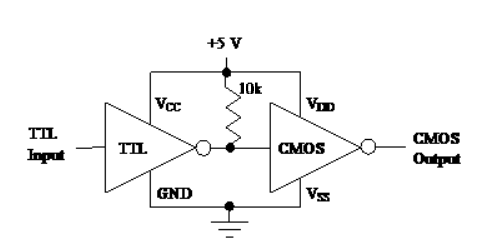
\includegraphics[scale=0.5]{figs/ej5/res_inter.png}
    \caption{Resistencia pull-up. Valor de referencia establecido en base a una alimentaci\'on com\'un de 5V (t\'ipica).}
    \label{ej5_fig:pull_up_res}
\end{figure}

\noindent
Otra posible soluci\'on es la utilizaci\'on de un integrado CD4504B\footnote{\href{https://www.ti.com/lit/ds/symlink/cd4504b-ep.pdf}{https://www.ti.com/lit/ds/symlink/cd4504b-ep.pdf}}, el cual se utiliza precisamente para estos casos, o el uso de un transistor BJT (permitiendo distintas alimentaciones) como se diagrama en la figura \ref{ej5_fig:transistor_inter}.

\begin{figure}[H]
    \centering
    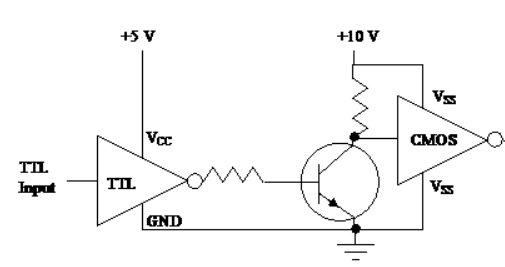
\includegraphics[scale=0.5]{figs/ej5/transistor_inter.png}
    \caption{Level Shifter mediante transistor NPN.}
    \label{ej5_fig:transistor_inter}
\end{figure}

\noindent
Existe otra soluci\'on interesante y es el caso del uso de un transistor BJT PNP entre ambas etapas, como se muestra en la figura \ref{ej5_fig:transistor_inter_pnp}. A su vez, otras posibles implementaciones incluyen transistores MOSFET o buffers TTL en la interconexi\'on. 

\begin{figure}[H]
    \centering
    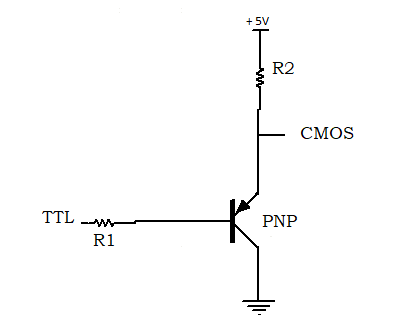
\includegraphics[scale=0.5]{figs/ej5/Levelshifter.png}
    \caption{Level Shifter mediante transistor PNP.}
    \label{ej5_fig:transistor_inter_pnp}
\end{figure}

\subsection{Implementaci\'on pr\'actica}
\noindent
Con el fin de llevar a cabo la presente experiencia, se decidi\'o utilizar un integrado digital 74LS08\footnote{\href{http://www.ti.com/lit/ds/symlink/sn74ls08.pdf}{http://www.ti.com/lit/ds/symlink/sn74ls08.pdf}} para la compuerta AND. Por su parte, para la compuerta OR se seleccion\'o un integrado digital 74HC32\footnote{\href{https://assets.nexperia.com/documents/data-sheet/74HC_HCT32.pdf}{https://assets.nexperia.com/documents/data-sheet/74HC_HCT32.pdf}}. En las respectivas hojas de datos se indica que la tensi\'on VOH m\'inima de la compuerta AND es de 2,4V y la VIH m\'inima de la compuerta OR es de 3,15V (con alimentaci\'on de 4,5V), pudiendo presentarse el problema ya descripto (ver \ref{ej5_ref:problema}).

\noindent
Como primera medida en la pr\'actica, se analizaron las salidas individuales de las compuertas encontr\'andose estas desconectadas entre s\'i. Para ello se aplicaron se\~nales cuadradas de 6Vpp a ambos bornes de entrada, generando valores de entrada altos y bajos alternadamente. Ante estas condiciones la salida deber\'ia tomar valores altos (tensi\'on mayor a VOH) y bajos (tensi\'on menor a VOL) respectivamente de acuerdo a la tensi\'on de entrada. En la figura \ref{ej5_fig:compuertas_desconectadas} se muestras las mediciones realizadas, ocurriendo efectivamente lo previsto.

\begin{figure}[H]
    \centering
    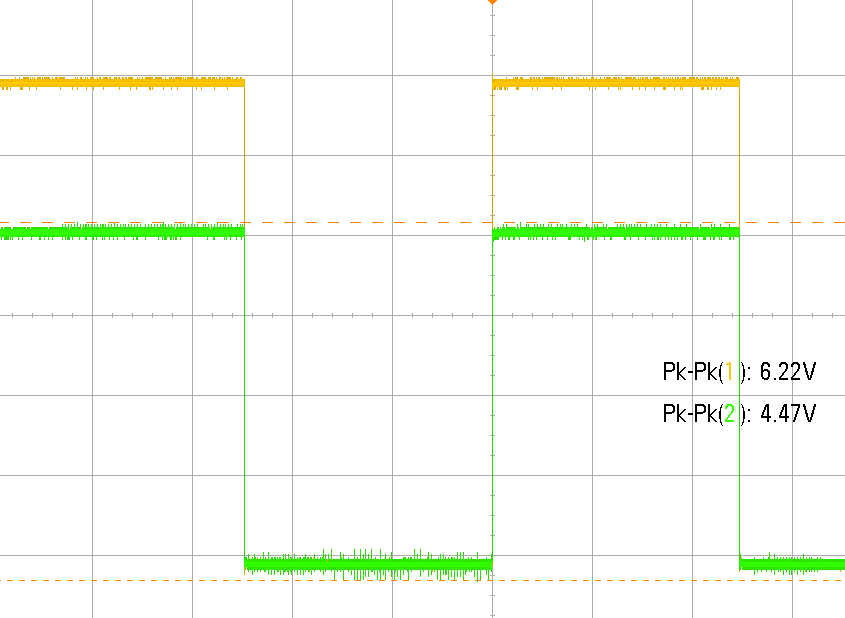
\includegraphics[width=.475\textwidth]{figs/ej5/and_cuadrada.png}\hfill
    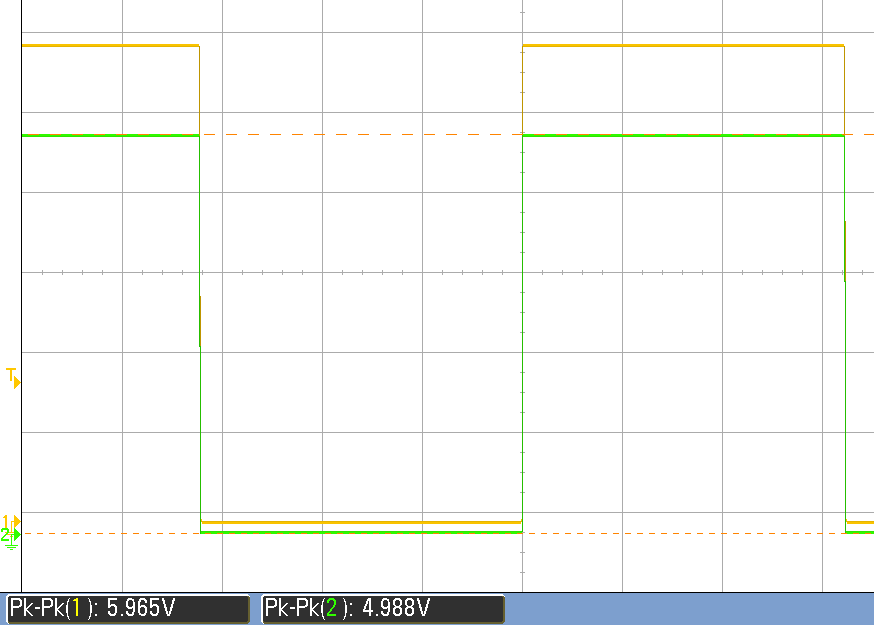
\includegraphics[width=.475\textwidth]{figs/ej5/or_cuadrada.png}
    \caption{Mediciones con las compuertas desconectadas.}
    \label{ej5_fig:compuertas_desconectadas}
    \subcaption{\footnotesize{*Izquierda: compuerta AND. Derecha: compuerta OR.}}
    \subcaption{\footnotesize{*Se\~nal amarilla: entrada. Se\~nal verde: salida.}}
\end{figure}

\noindent
Posteriormente, se realiz\'o el mismo procedimiento con las compuertas conectadas como en la figura \ref{ej5_fig:compuertasjuntas}. Al realizarlo, el circuito se comport\'o adecuadamente y no se registraron problemas por incompatibilidad. Sin embargo, bajo el prop\'osito de forzar su aparici\'on se carg\'o al circuito con una resistencia pull down entre ambas compuertas. Esto se realiz\'o ajustando el valor de un preset hasta que surgiera el error. Las mediciones se encuentran reflejadas en la figura \ref{ej5_fig:incompatibilidad}.

\begin{figure}[H]
    \centering
    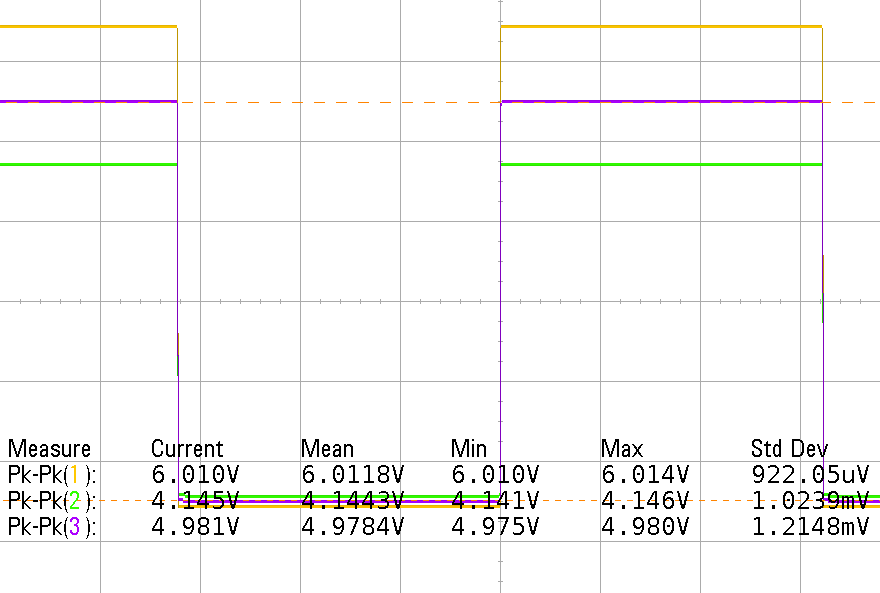
\includegraphics[width=.475\textwidth]{figs/ej5/andorsinres.png}\hfill
    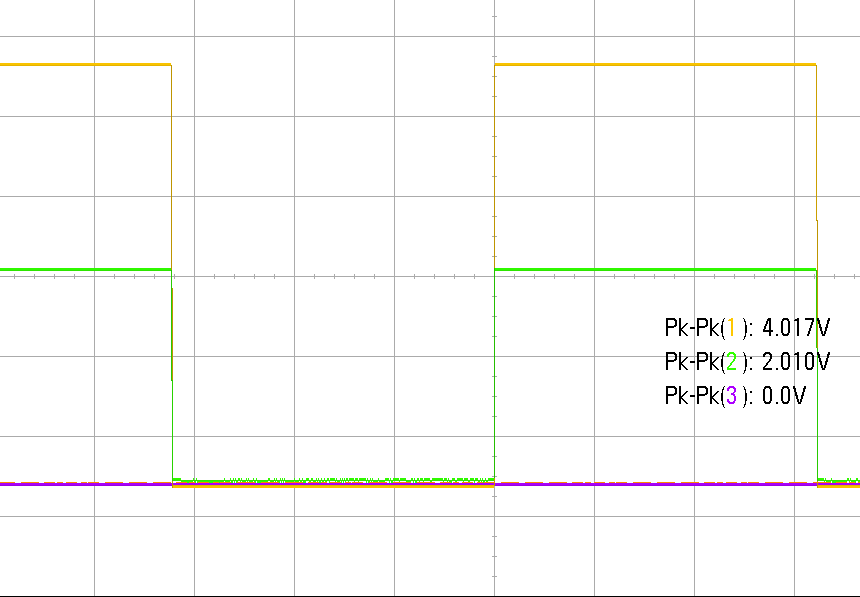
\includegraphics[width=.475\textwidth]{figs/ej5/pull_down.png}
    \caption{Mediciones con las compuertas conectadas.}
     \label{ej5_fig:incompatibilidad}
    \subcaption{\footnotesize{*Izquierda: respuesta del circuito. Derecha: incorporaci\'on de una carga.}}
    \subcaption{\footnotesize{*Se\~nal amarilla: entrada. Se\~nal violeta: etapa intermedia entre ambas compuertas. Se\~nal verde: salida.}}
   
\end{figure}

\noindent
Como soluci\'on ante dicho problema se incorpor\'o un level shifter mediante un transistor BJT PNP BC557 y dos resistores, de la forma diagramada en la figura \ref{ej5_fig:transistor_inter_pnp}, siendo R1 de 1k$\Omega$ y R2 de 10k$\Omega$. Esta etapa gener\'o un aumento en la tensi\'on de salida de la compuerta AND, resolviendo el problema de incompatibilidad. La salida en este caso se puede apreciar en la figura \ref{ej5_fig:pull_up}.

\begin{figure}[H]
    \centering
    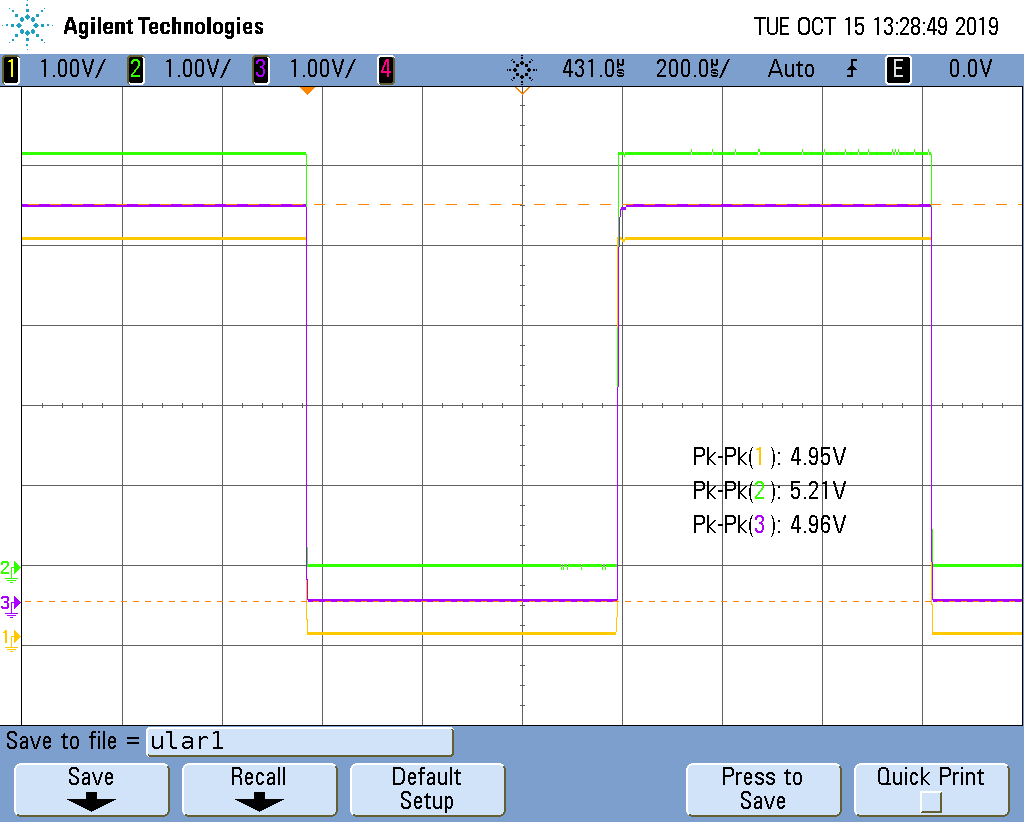
\includegraphics[width=0.6\textwidth]{figs/ej5/levelshifter10k1k.png}
    \caption{Resoluci\'on de la incompatibilidad mediante un level shifter.}
    \label{ej5_fig:pull_up}
\end{figure}
\subsection{Conclusiones}
\noindent
Mediante la presente experiencia, se analiz\'o la compatibilidad entre la conexi\'on de una salida TTL con una entrada CMOS. Se evidenci\'o que aunque en primera medida el circuito se comporte normalmente, pueden surgir problemas que son necesarios tener en cuenta.
\noindent
El problema mencionado se da por el hecho de que la tensi\'on de salida de una compuerta TTL puede ser menor que la tensi\'on VIH de una CMOS en estado alto. Con el fin de solucionar la problem\'atica, existen distintas opciones. En este caso, se incorpor\'o una etapa de lever shifting entre ambas compuertas, la cual di\'o lugar a un aumento de la tensi\'on de salida de la TTL, solventando el problema desarrollado.
\newpage
\section{Ejercicio 6}
\subsection{Introducci\'on}
\noindent
En esta sección se implementará un Latch SR y un Flip Flop D mediante compuertas lógicas en una placa PCB, para luego encontrar conclusiones relevantes sobre las mismas y compararlas con los valores de las compuertas comerciales.
%
\subsection{Latch SR}
\subsubsection{Funcionamiento}
\noindent
Un Latch SR es un circuito encargado de almacenar un valor permitiendo borrar al mismo, es decir actúa como una memoria de 1 bit que permite almacenar o borrar su valor según el valor de sus entradas, para esto presenta una entrada denominada usualmente como Set que se encarga de fijar el valor que se querrá almacenar (cero o uno) y una entrada Reset que se encarga de borrar el valor almacenado haciendo que el mismo valga cero para cualquier valor de set.
%
\subsubsection{Circuito implementado}
\noindent
De esta manera el circuito típico correspondiente al Latch SR se muestra en la figura \ref{ej6_latch_sr} y la tabla de verdad del mismo se puede apreciar en la tabla \ref{ej6_tabla_latch_sr}. \\
%
La entrada S corresponde a la entrada Set y la entrada R refiere a la entrada Reset.
%
%
%
\begin{figure}[H]
    \centering
        \centering
        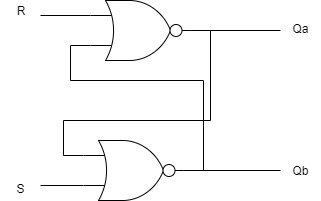
\includegraphics[width=0.5\textwidth]{figs/Ej6/latchsr.jpg} % first figure itself
         \caption{Circuito correspondiente a un Latch SR}
         \label{ej6_latch_sr}
\end{figure}
%
\begin{table}[H]
\caption{Tabla de verdad correspondiente al Latch SR (donde $Qa_{-1}$ refiere al valor que se almacena en el latch.}
\label{ej6_tabla_latch_sr}
\centering
\begin{tabular}{|l|l||l|l|}
\hline
S & R & Qa & Qb \\ \hline \hline
0   & 0     & $Qa_{-1}$     & $Qb_{-1}$     \\ \hline
0   & 1     & 0     & 1   \\ \hline
1   & 0    & 1     & 0   \\ \hline
1   & 1    & 0     & 0   \\ \hline 
\end{tabular}
\end{table}
%
\noindent
De esta forma se trabajó con compuertas NOR para la creación del Latch, para eso se consideró interesante trabajar con compuertas lógicas CD4001B, ya que las mismas son más lentas que las compuertas 74HC02 y hay mayor disponibilidad de ellas en el pañol de la facultad. Las hojas de datos de dichas compuertas se pueden encontrar en los siguientes links \href{http://www.ti.com/lit/ds/symlink/cd4001b-mil.pdf}{CD4001b}, \href{http://www.ti.com/lit/ds/symlink/sn74hc02.pdf}{74HC02}.
%
\subsubsection{Mediciones y Conclusiones.}
%
\noindent
Así se midió el cambio en la salida cuando Reset esta en cero y Set cambia de 0 a 1, de esta forma, en las figuras \ref{ej6_latch_imagen1} y \ref{ej6_latch_imagen2} presentadas a continuación se pueden ver el tiempo de rise y el tiempo de propagación para estas compuertas en estas condiciones. Cabe destacar que la medición de estos valores se realizó con puntas x10 debido a que la medición con puntas x1 se veía muy alterada por el instrumento de medición.
\noindent
\begin{figure}[H]
    \centering
        \centering
        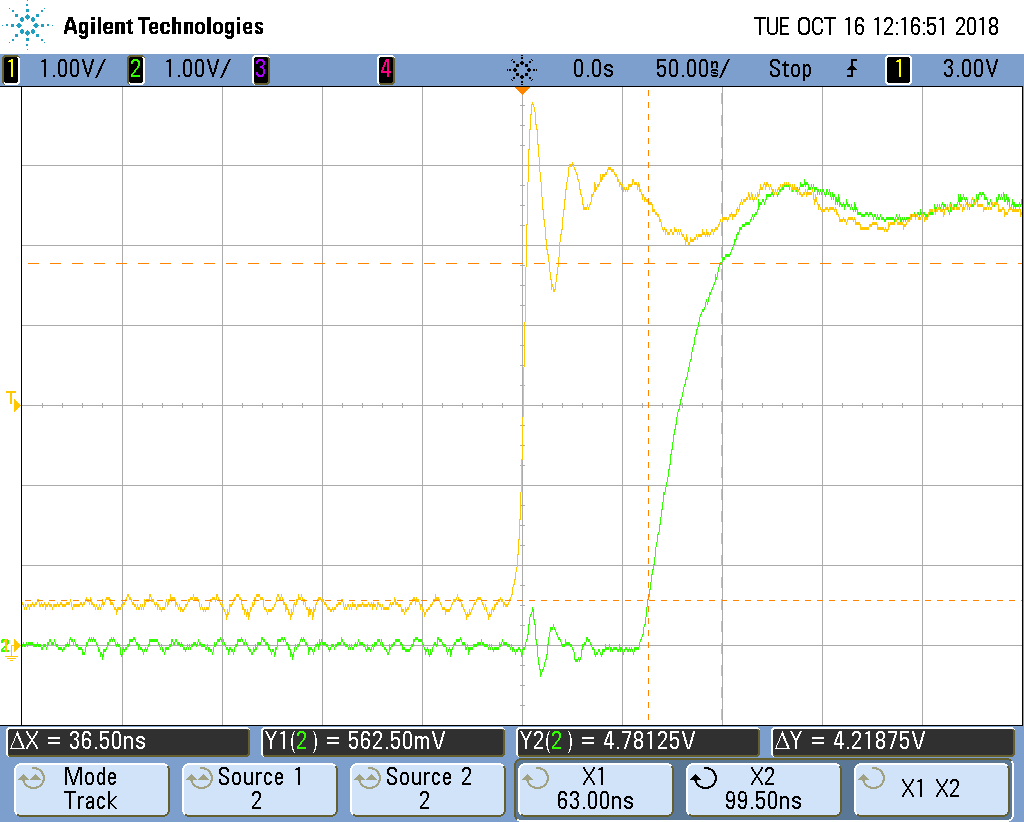
\includegraphics[width=0.6\textwidth]{figs/Ej6/sr_trise.png} % first figure itself
         \caption{Medición correspondiente al tiempo de rise de la compuerta.}
         \label{ej6_latch_imagen1}
\end{figure}
%
%
\begin{figure}[H]
    \centering
        \centering
        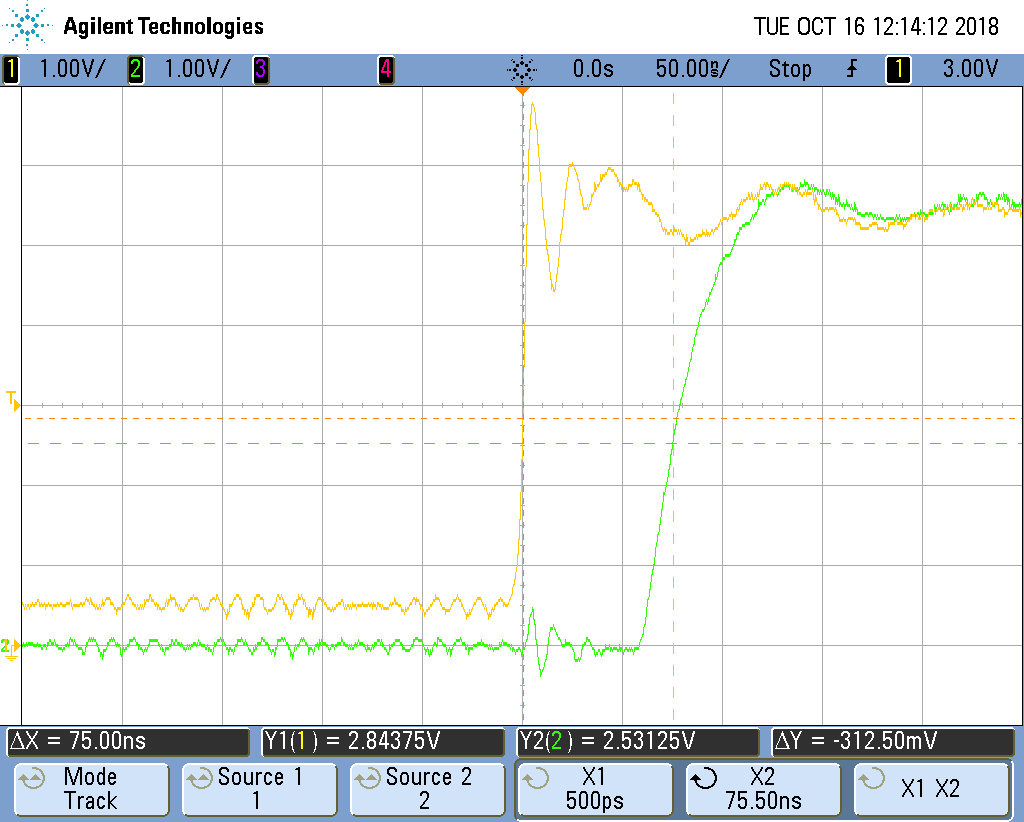
\includegraphics[width=0.6\textwidth]{figs/Ej6/sr_tplhx10.png} % first figure itself
         \caption{Medición correspondiente al tiempo de propagaci\'on de la compuerta.}
         \label{ej6_latch_imagen2}
\end{figure}
%
\noindent
De forma análoga se midieron los tiempos de fall y de propagación al pasar de 1 a cero en la salida es decir con set en 0 y reset en 1.\\
%
\noindent
Así, los tiempos que se obtuvieron se muestran en la tabla \ref{ej6_tabla_mediciones_latch} junto con los tiempos de una compuerta representativa de un latch SR comercial, de esta forma, para la comparación se utilizó la compuerta M74HC279C1R de la marca ST, la hoja de datos de la misma se puede encontrar en el siguiente link \href{http://pdf.datasheetcatalog.com/datasheets2/24/245012_1.pdf}{74HC279}.
%
\begin{table}[H]
\caption{Tabla con los valores de las mediciones tomadas (valores en nano segundos)}
\label{ej6_tabla_mediciones_latch}
\centering
\begin{tabular}{|l||l|l|l|l|}
\hline 
            & $T_{PLH}$ & $T_{PHL}$ & $T_{rise}$ & $T_{fall}$ \\ \hline \hline
Circuito    & 75        & 70        & 36.5       & 30         \\ \hline
M74HC279C1R & 20        & 20        & 15         & 15         \\ \hline
\end{tabular}
\end{table}
%
\noindent
En la tabla $T_{PLH}$ y $T_{PHL}$ refieren a los tiempos de propagación al cambiar S a uno o R a uno respectivamente.\\
Podemos ver que los valores obtenidos presentan diferencias con los valores encontrados comúnmente en la práctica, esto tiene sentido debido a que sabíamos que las compuertas utilizadas para la medición eran lentas comparadas con otras compuertas disponibles. De todas formas vemos que las mediciones se encuentran en el orden de magnitud de los valores de los componentes encontrados comercialmente.
%
\subsection{Flip Flop D}
%
\subsubsection{Funcionamiento}
\noindent
Un flip flop D se encarga de almacenar un bit, al igual que en el caso anterior, sólo que tiene una única entrada (D) y un controlador que le indica en que momento tomar el dato de dicha entrada, es decir el sistema se conecta a un clock (Clk) que le indica cuándo almacenar el valor de la entrada D.
%
\subsubsection{Circuito implementado}
\noindent
Por la naturaleza del sistema, el mismo presenta un latch SR en su interior, esto se puede ver en el esquemático del correspondiente circuito en la figura \ref{ej6_flip_flop_D}. Además posee un Edge Detector, que se encarga de detectar los flancos positivos o negativos, según sea la naturaleza del flip flop, el esquemático del mismo se encuentra en la figura \ref{ej6_flip_flop_D_edge}, el mismo corresponde a un detector de flancos negativos, se decidió por esta alternativa debido a la simpleza de implementación utilizando para realizarla un único integrado.
%
%
\begin{figure}[H]
    \centering
        \centering
        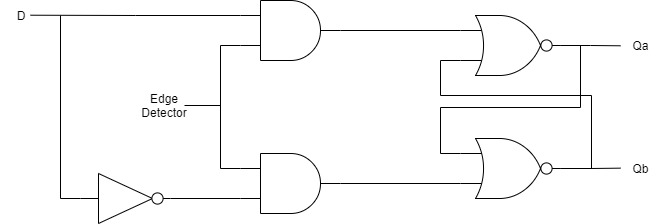
\includegraphics[width=0.8\textwidth]{figs/Ej6/flipflop.jpg} % first figure itself
         \caption{Circuito característico del Flip flop}
         \label{ej6_flip_flop_D}
\end{figure}
%
\begin{figure}[H]
    \centering
        \centering
        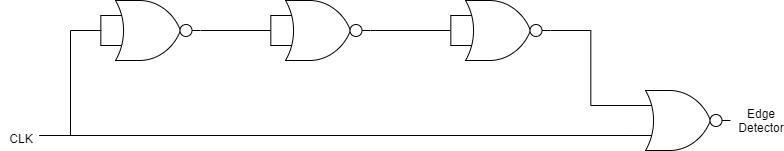
\includegraphics[width=0.8\textwidth]{figs/Ej6/Edgedetetor.jpg} % first figure itself
         \caption{Circuito implementado para la detección de flancos con pendiente negativa.}
         \label{ej6_flip_flop_D_edge}
\end{figure}
%
\noindent
De esta manera la tabla de verdad de dicho circuito se puede ver en la tabla \ref{ej6_tabla_flip_flop_D}
%
%
\begin{table}[H]
\caption{Tabla de verdad correspondiente al Flip Flop D}
\label{ej6_tabla_flip_flop_D}
\centering
\begin{tabular}{|l|l||l|l|}
\hline
D & CLK                     & Qa         & Qb         \\ \hline
0 & $\downarrow$ & 0          & 1          \\ \hline
1 & $\downarrow$ & 1          & 0          \\ \hline
X & X                       & $Qa_{-1}$ & $Qb_{-1}$ \\ \hline
\end{tabular}
\end{table}
%
\noindent
De esta manera para implementar al circuito en placa PCB se decidió utilizar los integrados 74HC08 para las compuertas And, 74HC00 para las compuertas Nand y 74HC02 para las compuertas Nor, utilizando una compuerta nor para la compuerta not que requiere el flip flop, como se puede ver en la figura \ref{ej6_flip_flop_D}. Las hojas de datos de los componentes utilizados se pueden consultar en los siguientes links \href{http://www.ti.com/lit/ds/symlink/sn74hc08.pdf}{74HC08}, \href{http://www.ti.com/lit/ds/symlink/sn74hc02.pdf}{74HC02}, \href{http://www.ti.com/lit/ds/symlink/sn74hc00.pdf}{74HC00}.
%

\subsubsection{Mediciones y Conclusiones}
\noindent
De esta manera se procedió análogamente al caso del latch SR, es decir, se midieron los tiempos de subida y bajada a la salida de la compuerta, considerando (al igual que en el caso anterior) que el tiempo de rise o subida comienza cuando la salida vale 10\% del valor tomado como High y termina cuando vale 90\% del valor tomado como High. El caso del tiempo de bajada es análogo pero a la inversa, es decir comienza cuando la salida es 90\% del valor High y finaliza cuando el mismo es del 10\% del valor de High.\\
%
También es análogo el tratamiento de los tiempos de propagación del circuito, sólo que aquí la entrada que cambia es D es decir cuando D cambia de cero a uno se obtiene el tiempo de propagación $T_{PLH}$ y cuando la entrada D cambia de uno a cero se obtiene $T_{PHL}$, ambos tiempos medidos como en la figura \ref{ej6_latch_imagen2}, es decir desde que la señal de input alcanza el 50\% de su valor considerado como high hasta que la señal de salida del sistema llega al 50\% de su valor considerado como high.\\
%
Para los valores correspondientes a un flip flop D comercial, se decidió contrastar las mediciones tomadas con el flip flop D 74HC74, se optó por el mismo ya que se encuentra en el pañol de la facultad y es el equivalente al utilizado en el ejercicio 7 (74LS74) pero que trabaja con la misma tecnología que las compuertas utilizadas en nuestro caso, a saber, tecnología CMOS. Si bien cabe destacar que el SN74HC74 es de flanco positivo mientras que nuestro flip flop D es de flanco negativo. La hoja de datos del componente se puede revisar en el siguiente link \href{http://www.ti.com/lit/ds/symlink/sn74hc74-ep.pdf}{74HC74}.\\
De esta manera los resultados obtenidos de las mediciones del circuito y los que se pueden encontrar en la hoja de datos del SN74HC74 se muestran en la tabla \ref{ej6_tabla_flip_flop_mediciones}.
%
\begin{table}[H]
\caption{Valores medidos para el circuito junto a los encontrados para el Flip Flop D SN74HC74.}
\label{ej6_tabla_flip_flop_mediciones}
\centering
\begin{tabular}{|l||l|l|l|l|}
\hline
    & $T_{PLH}$ & $T_{PHL}$ & $T_{rise}$ & $T_{fall}$ \\ \hline \hline
Circuito & 20        & 20        & 6          & 6          \\ \hline
SN74HC74 & 29        & 31        & 44         & 41         \\ \hline
\end{tabular}
\end{table}
%
\noindent
Se puede apreciar que existe una notoria diferencia entre el tiempo de rise y fall del circuito medido respecto de lo que se esperaría obtener en el integrado comercial, esto puede deberse a múltiples factores que pueden estar mejor resueltos en el integrado, debido a la cercanía de sus componentes y la facilidad del fabricante de controlar los parámetros de cada etapa a su necesidad. Además las puntas del osciloscopio hacen que la medición de dichos tiempos tan cortos se vean drásticamente modificadas, esto ya se vió en la sección destinada al Latch SR, en donde el tiempo de propagación medido con puntas x10 fue de 75ns pero medido con puntas x1 fue de 147ns.   
Con respecto a los tiempos de propagaci\'on la diferencia se encuentra dentro de lo esperado debido a las ventajas ya mencionadas que presenta el fabricante a la hora de diseñar el integrado.
\newpage
\section{Ejercicio 7}

\subsection{Introducci\'on}
\noindent
En la presente sección se desarrolla la implementaci\'on de dos contadores de 3 bits, uno sincr\'onico y otro asincr\'onico. Se analizan diferencias de funcionamiento entre ambos y se cuantifica la m\'axima velocidad de operaci\'on de cada uno. 

\subsection{Diseño}
\noindent
A continuaci\'on se explican los circuitos utilizados para cada implementaci\'on.

\subsubsection{Contador asincr\'onico}
\label{ej7_sec:cont_asinc}
\noindent
Para la implementaci\'on del contador asincr\'onico se parte del circuito de la Figura 	\ref{ej7_fig:asinc_init}. Tomando N = $Q_2 Q_1 Q_0$, este contador cuenta de 0 a 7 y luego vuelve a comenzar. Se trata de un contador
asincr\'onico porque, como se puede observar, s\'olo el primer Flip-Flop tiene su entrada de CLK conectada a la señal de clock, mientras que los dem\'as se activan con un flanco ascendente de $\overline{Q_{n-1}}$, es decir, un flanco descendente de $Q_{n-1}$. Por lo tanto, tomando como ejemplo el caso de que tenga que activarse el \'ultimo Flip-Flop, a \'este le llega el flanco ascendente luego del retardo de los dos primeros, con lo que no hay sincronismo. \\
%
\begin{figure}[H]
	\centering
	\resizebox{0.7\linewidth}{!}{
			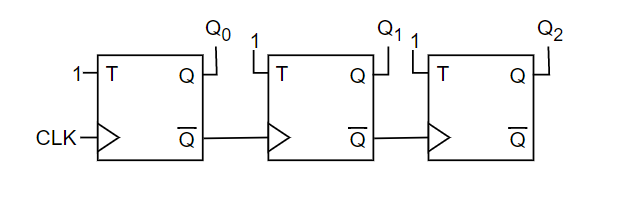
\includegraphics{figs/ej7/ej7_asinc_circ.PNG}	
	}
	\caption{Circuito de un contador asincr\'onico de 3 bits.}
	\label{ej7_fig:asinc_init}
\end{figure}
%
\noindent
Como solamente se dispone de circuitos integrados Flip-Flop D, se utilizan \'estos para obtener los Flip-Flop T que utiliza el circuito. Para ello, se busca una funci\'on l\'ogica que relacione la entrada T y la salida Q con la entrada D que debe tener el integrado para que el circuito se comporte como un Flip-Flop T. La tabla de verdad de dicha funci\'on se muestra en la Tabla \ref{ej7_tab:FFDaFFT}.
%
\begin{table}[H]
\centering
\begin{tabular}{|c|c|c|}
\hline
\textbf{T} & \textbf{Q} & \textbf{D} \\ \hline
0          & 0          & 0          \\ \hline
0          & 1          & 1          \\ \hline
1          & 0          & 1          \\ \hline
1          & 1          & 0          \\ \hline
\end{tabular}
\caption{Tabla de verdad para hacer un FFT a partir de un FFD.}
\label{ej7_tab:FFDaFFT}
\end{table}
%
\noindent
De la tabla de verdad se obtiene que:
%
\begin{equation}
	D = T \oplus Q
\end{equation}
%
Por lo tanto, se obtiene un Flip-Flop T a partir de un Flip-Flop D mediante el circuito de la Figura \ref{ej7_fig:FFDaFFT}.
%
\begin{figure}[H]
	\centering
	\resizebox{0.5\linewidth}{!}{
		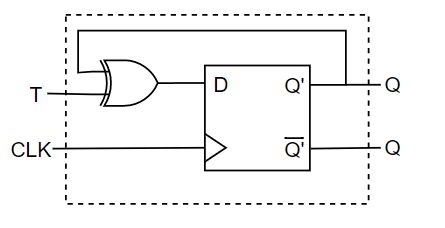
\includegraphics{figs/ej7/ej7_ffd_fft.PNG}
	}
	\caption{Circuito para hacer un FFT a partir de un FFD.}
	\label{ej7_fig:FFDaFFT}
\end{figure}
%
\noindent
Por lo tanto, el circuito definitivo a implementar para el contador sincr\'onico es el de la Figura \ref{ej7_fig:AsincFinal}

%
\begin{figure}[H]
	\centering
	\resizebox{0.9\linewidth}{!}{
		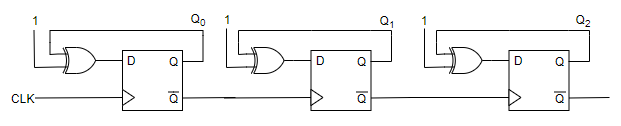
\includegraphics{figs/ej7/ej7_ffd_asinc.PNG}
	}
	\caption{Contador asincr\'onico con FFD.}
	\label{ej7_fig:AsincFinal}
\end{figure}
%
\subsubsection{Contador sincr\'onico}
\noindent
Para el contador asincr\'onico, se parte del contador de la Figura \ref{ej7_fig:sinc_circ}, donde como todos los Flip-Flops est\'an conectados a la señal de clock, se evidencia el sincronismo que le da el nombre a este tipo de contadores. Se trata al igual que en el caso anterior de un contador de 3 bits que cuenta de 0 a 7 y se reinicia. Se incluye en el circuito el bit Z, que vale 1 en el tick anterior a que se reinicie el contador, podr\'ia ser de utilidad dependiendo de la aplicaci\'on.
%
\begin{figure}[H]
	\centering
	\resizebox{0.8\linewidth}{!}{
		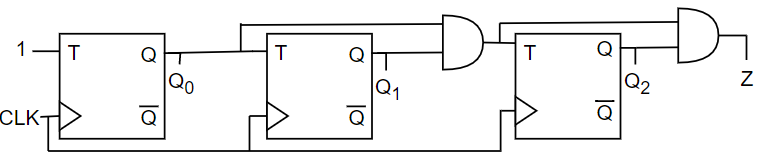
\includegraphics{figs/ej7/ej7_sinc_circ.PNG}
	}
	\caption{Circuito contador sincr\'onico de 3 bits.}
	\label{ej7_fig:sinc_circ}
\end{figure}
%
\noindent
Al igual que en la Subsecci\'on \ref{ej7_sec:cont_asinc}, se utilizan Flip-Flops D para realizar las Flip-Flops T, de modo que el circuito definitivo es el de la Figura \ref{ej7_fig:sinc_circ_final}.
%
\begin{figure}[H]
	\centering
	\resizebox{\linewidth}{!}{
		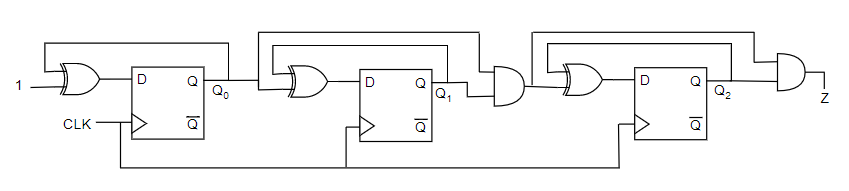
\includegraphics{figs/ej7/ej7_sinc_circ_final.PNG}
	}
	\caption{Circuito del contador sincr\'onico con FFD.}
	\label{ej7_fig:sinc_circ_final}
\end{figure}
%
\subsubsection{Implementaci\'on}
\noindent
Antes de la realizaci\'on se simul\'o el circuito en Proteus para verificar su correcto funcionamiento, en la Figura \ref{ej7_fig:sim_proteus} se muestra la simulaci\'on.
%
\begin{figure}[H]
	\centering
	\resizebox{0.8\linewidth}{!}{
		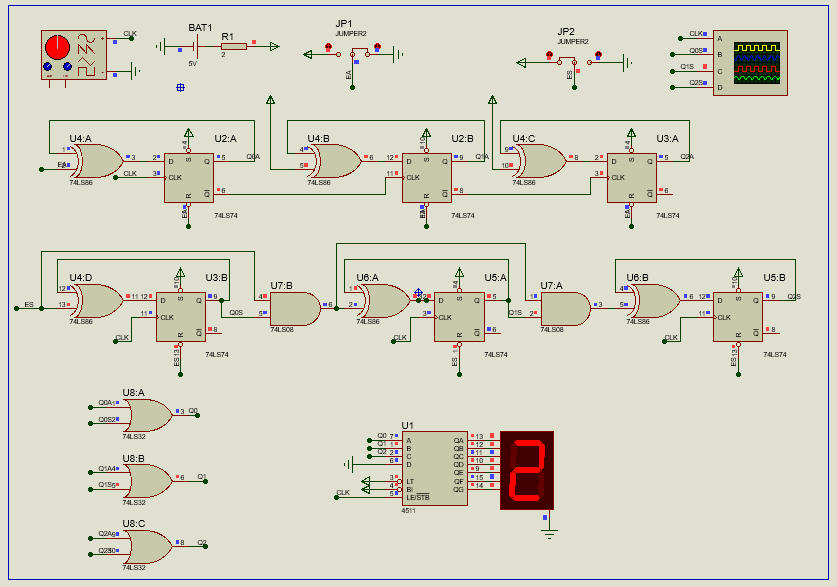
\includegraphics{figs/ej7/ej7_sim_proteus.PNG}
	}
	\caption{Simulaci\'on en Proteus.}
	\label{ej7_fig:sim_proteus}
\end{figure}
%
\noindent
Para la implementaci\'on de los contadores se utilizan compuertas AND, XOR y Flip-Flops D de tecnolog\'ia Low Shottky TTL y se muestra la cuenta en un display LED 7 segmentos. En la Figura \ref{ej7_fig:placa_andando} se muestra una captura de las placas andando.
%
\begin{figure}[H]
	\centering
	\resizebox{0.9\linewidth}{!}{
		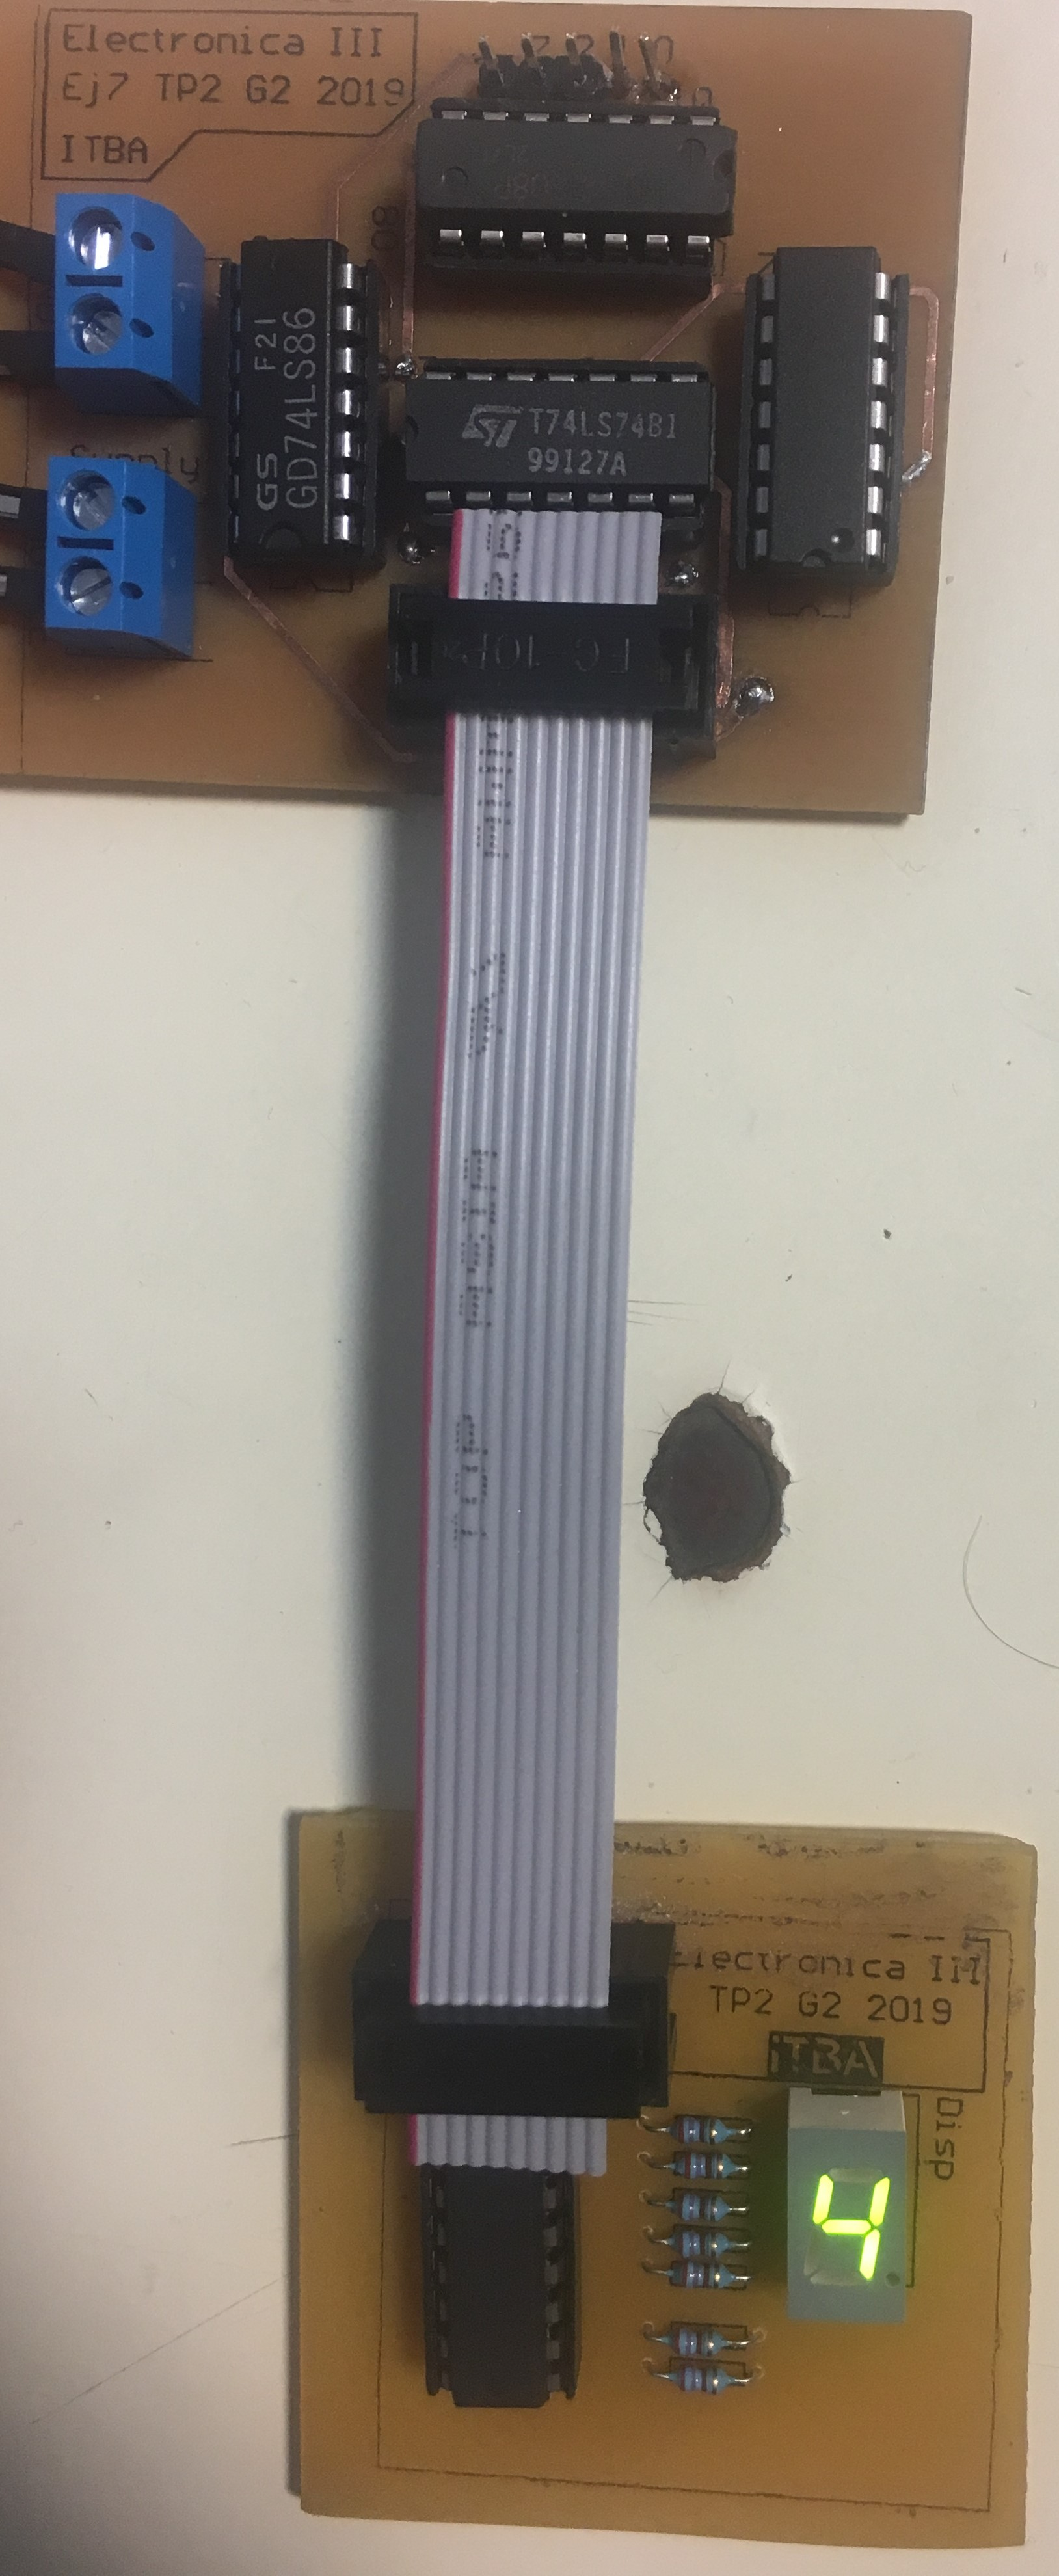
\includegraphics[angle = 90]{figs/ej7/circ_andando.jpeg}
	}
	\caption{Implementaci\'on.}
	\label{ej7_fig:placa_andando}
\end{figure}
%
\subsection{An\'alisis de resultados}
\noindent
A continuaci\'on se muestran las mediciones del funcionamiento de cada contador y sus correspondientes tiempos de propagaci\'on, a partir de los cuales se puede obtener la m\'axima velocidad de operaci\'on.
%
\subsubsection{Contador asincr\'onico}
\label{ej7_sec:meas_cont_asinc}
\noindent
%En la Figura \ref{} se muestra el funcionamiento del contador asincr\'onico,
En el caso del contador asincr\'onico, se mide el tiempo entre los flancos ascendentes del clock y la respuesta de la señal $Q_2$, que por acarrear los retardos de los otros dos Flip-Flops, es el que mayor retardo presenta. \'Esto se puede comprobar en la Figura \ref{ej7_fig:asinc_0vs2}, donde se observan la señal de clock, los bits $Q_0$ y $Q_2$, y se puede apreciar c\'omo \'este \'ultimo presenta un tiempo de propagaci\'on mayor desde el flanco ascendente de la señal de clock.
%
\begin{figure}[H]
	\centering
	\resizebox{0.7\linewidth}{!}{
		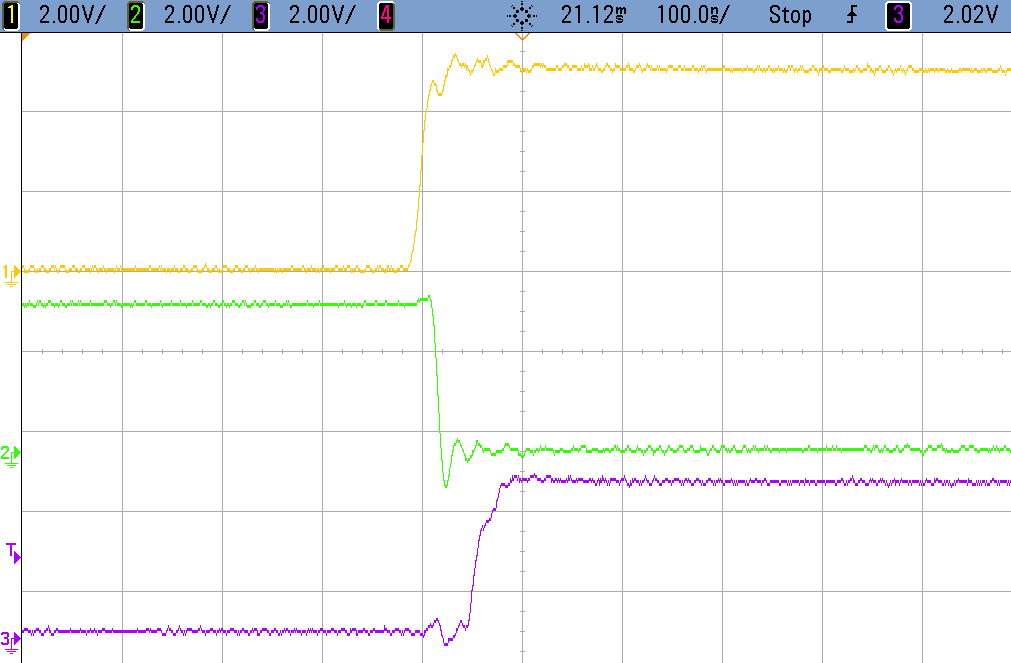
\includegraphics{figs/ej7/cont_asinc_0vs2.png}
	}
	\caption{Clock (amarillo), $Q_0$ (verde) y $Q_2$ (violeta).}
	\label{ej7_fig:asinc_0vs2}
\end{figure}
%
\noindent
Para la medici\'on del tiempo de retardo, se mide el tiempo desde que la señal de clock vale el promedio entre su valor bajo y alto, hasta que la salida toma el valor $V_{OH}$. Para fijar los valores de tensi\'on necesarios para medir, se miden los par\'ametros mencionados del clock, y se busca el valor m\'inimo de $V_{OH}$ en la \href{https://www.ti.com/lit/ds/symlink/sn74s74.pdf}{hoja de datos del fabricante}. Dichos valores se muestran en la Tabla \ref{ej7_tab:valores_medicion}.
%
\begin{table}[H]
\centering
\begin{tabular}{|c|c|}
\hline
\textbf{Par\'ametro} & \textbf{Valor {[}V{]}} \\ \hline
$V_{CLK0}$       & 25m                  \\ \hline
$V_{CLK1}$       & 5,1                    \\ \hline
$V_{CLK50\%}$    & 2,5625                 \\ \hline
$V_{OH}$         & 2,7                    \\ \hline
\end{tabular}
\caption{}
\label{ej7_tab:valores_medicion}
\end{table}
%
\noindent
 Por lo tanto, se mide el tiempo entre que la entrada vale $2,5625V$ hasta que la salida vale $2,7V$. En la Figura \ref{ej7_fig:asinc_measure1} se muestra la medici\'on del tiempo de retardo del bit $Q_2$, de donde se tiene que:
 \begin{equation*}
     t_P = 63,3ns
 \end{equation*} 
%
\begin{figure}[H]
	\centering
	\resizebox{0.8\linewidth}{!}{
			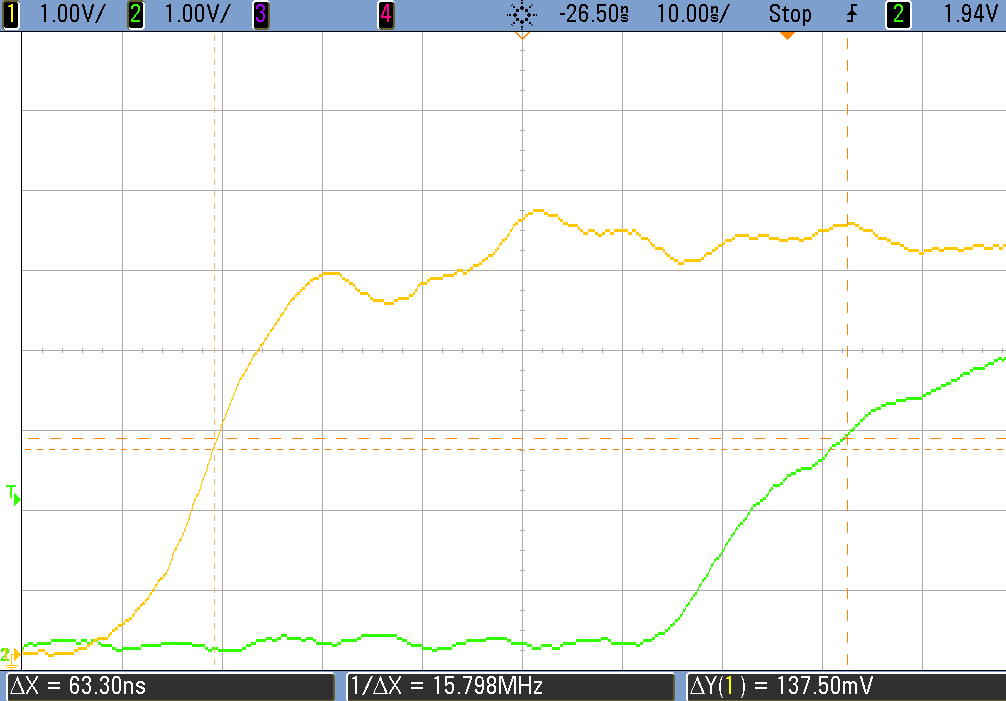
\includegraphics{figs/ej7/cont_asinc_tprop.png}	
	}
	\caption{Medici\'on del tiempo de retardo del contador asincr\'onico.}
	\label{ej7_fig:asinc_measure1}
\end{figure}
%
\noindent
El valor medido est\'a dentro de lo esperado ya los tiempos de propagaci\'on t\'ipicos de los Flip-Flop, $t_{PLH}$ y $t_{PHL}$, son de 14$ns$ y 20$ns$, respectivamente. Teniendo en cuenta que cuando $Q_2$ se activa, $Q_0$ y $Q_1$ pasan al nivel bajo, el tiempo de propagaci\'on del circuito para Flip-Flops t\'ipicos ser\'ia de:
 \begin{equation}
     t_{TIP} = t_{PLH}\cdot 2 t_{PHL} = 74ns
 \end{equation}
 Teniendo el tiempo de propagaci\'on, para determinar la velocidad m\'axima de operaci\'on se pueden tomar distintos criterios. En \'este caso se busca asegurar una velocidad m\'axima para la cual la salida del contador tenga un valor estable en los flancos descendentes de clock, para que al utilizar \'este contador se pueda detectar leer la salida de forma sincr\'onica. Tomando \'este criterio, la m\'axima frecuencia de operaci\'on viene dada por:
 \begin{equation}
     f_{max} = \frac{1}{2\cdot t_{P}} = 7,9MHz
     \label{ej7_eq:vel_max}
 \end{equation}
\subsubsection{Contador sincr\'onico}
\noindent
En la Figura \ref{ej7_fig:sinc_allbits} se encuentra la señal de clock y los 3 bits del contador para la cuenta de 0 a 7, se muestra qu\'e valor toma la cuenta en cada per\'iodo de la señal de clock.
%
\begin{figure}[H]
	\centering
	\resizebox{0.8\linewidth}{!}{
			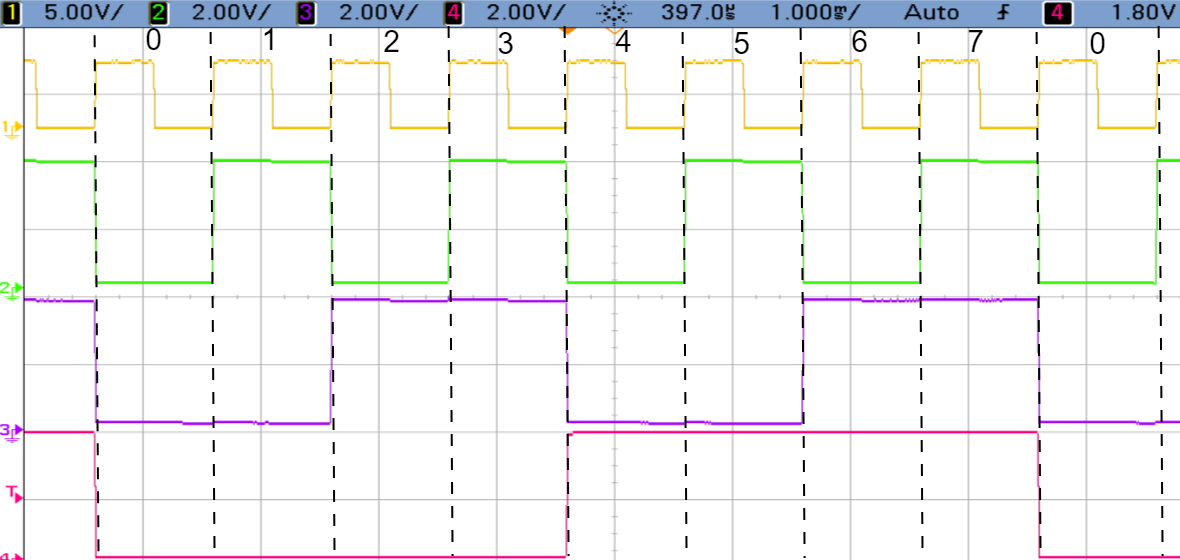
\includegraphics{figs/ej7/cont_sinc_allbits2.png}	
	}
	\caption{Señal de clock (amarillo) y los 3 bits del contador.}
	\label{ej7_fig:sinc_allbits}
\end{figure}
%
\noindent
Para la medici\'on se toman los mismos par\'ametros que en la Subsecci\'on \ref{ej7_sec:meas_cont_asinc}. En la Figura \ref{ej7_fig:sinc_q0_meas} se muestra la medici\'on del tiempo de propagaci\'on del bit $Q_0$, que es de 32,8$ns$. 
%
\begin{figure}[H]
	\centering
	\resizebox{0.8\linewidth}{!}{
			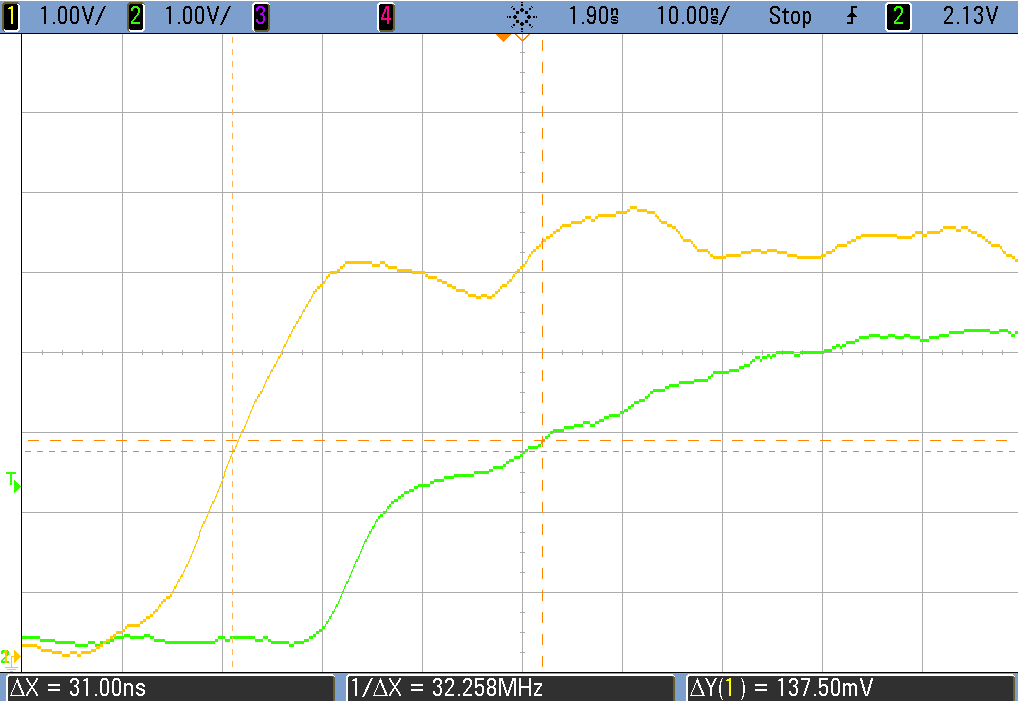
\includegraphics{figs/ej7/cont_sinc_q0_tprop.png}	
	}
	\caption{Medici\'on del tiempo de propagaci\'on del bit $Q_0$ del contador sincr\'onico.}
	\label{ej7_fig:sinc_q0_meas}
\end{figure}
\noindent
El valor del tiempo de propagaci\'on es mayor al esperado de los datos del fabricante, ya que deber\'ia ser menor al $t_{PLH}$ m\'aximo, 25$ns$. Sin embargo, se atribuye la diferencia de 7$ns$ al error de medici\'on, ya que la salida
del circuito no tomaba un valor estable, sino que cambiaba mucho y para la medici\'on se utiliz\'o una sola curva.
Si bien por ser sincr\'onico \'este tiempo deber\'ia ser igual para los 3 bits, se midieron los otros dos bits de la misma forma y se obtuvieron los valores de la Tabla \ref{ej7_tab:t_prop_all}.
%
\begin{table}[H]
\centering
\begin{tabular}{|c|c|}
\hline
\textbf{Bit} & \textbf{$t_p$(ns)} \\ \hline
$Q_0$           & 32,8            \\ \hline
$Q_1$           & 31              \\ \hline
$Q_2$           & 38,1            \\ \hline
\end{tabular}
\caption{Tiempo de propagaci\'on de cada bit del contador sincr\'onico.}
\label{ej7_tab:t_prop_all}
\end{table}
%
\noindent
De los valores medidos, el retardo de $Q_2$ determina la m\'axima velocidad de operaci\'on por ser el mayor. Adoptando el mismo criterio que en el contador asincr\'onico, para la m\'axima velocidad de operaci\'on del contador se obtiene mediante la Ecuaci\'on \ref{ej7_eq:vel_max} que:
\begin{equation*}
    f_{max} = 13,12MHz
\end{equation*}
%
\subsection{Resumen y conclusi\'on}
\noindent
En la siguiente tabla se muestran los valores obtenidos en las mediciones de cada contador.
%
\begin{table}[H]
\centering
\begin{tabular}{|c|c|c|}
\hline
\textbf{Contador} & \textbf{$t_{p}$} & \textbf{$f_{max}$} \\ \hline
Asincr\'onico       & 63,3$ns$           & 7,9$MHz$          \\ \hline
Sincr\'onico        & 38,1$ns$           & 13,12$MHz$        \\ \hline
\end{tabular}
\end{table}
\noindent
Como se esperaba a priori, se observ\'o que el contador sincr\'onico presenta un menor tiempo de propagaci\'on, por lo que en caso de querer trabajar en frecuencias muy altas es importante tener \'esto en cuenta. 
\newpage
\input{sections/conclusion.tex}
\end{document}